
\documentclass{article}

\IfFileExists{PRIMEarxiv.sty}{\usepackage{PRIMEarxiv}}{}

\usepackage[utf8]{inputenc}
\usepackage[T1]{fontenc}
\usepackage[hidelinks,hypertexnames=false]{hyperref}
\usepackage{url}
\usepackage{booktabs}
\usepackage{amsfonts}
\usepackage{amsmath}
\usepackage{amssymb}
\usepackage{nicefrac}
\usepackage{microtype}
\usepackage{fancyhdr}
\usepackage{graphicx}
\usepackage{array}
\usepackage{float}
\usepackage{caption}
\usepackage{titlesec}
\titlespacing*{\section}{0pt}{3.25ex plus 1ex minus .2ex}{1.25ex plus .2ex}
\titlespacing*{\subsection}{0pt}{1.5ex plus .6ex minus .2ex}{0.85ex plus .2ex}
\setlength{\textfloatsep}{6pt plus 2pt minus 2pt}
\setlength{\floatsep}{6pt plus 2pt minus 2pt}
\setlength{\intextsep}{5pt plus 2pt minus 2pt}
\setlength{\abovecaptionskip}{4pt}
\setlength{\belowcaptionskip}{4pt}
\captionsetup{skip=4pt}
\newenvironment{mainresultstight}{%
  \begingroup
  \setlength{\parskip}{0pt plus 0pt minus 0pt}%
  \titlespacing*{\section}{0pt}{0pt}{1.4ex}%
  \titlespacing*{\subsection}{0pt}{1.4ex}{1.65ex}%
}{%
  \par\vfill
  \endgroup
  \titlespacing*{\section}{0pt}{3.25ex plus 1ex minus .2ex}{1.25ex plus .2ex}%
  \titlespacing*{\subsection}{0pt}{1.5ex plus .6ex minus .2ex}{0.85ex plus .2ex}%
}
\graphicspath{{paper_figures/}}

\pagestyle{fancy}
\thispagestyle{empty}
\rhead{\textit{}}
\fancyhead[LO]{Wayfinder Attention}

\providecommand{\keywords}[1]{\par\noindent\textbf{Keywords: }#1}
\providecommand{\and}{, }
\newcommand{\methodname}{Wayfinder Attention}
\newcommand{\topk}{\operatorname{TopK}}
\newcommand{\recall}{\operatorname{Recall}}

\title{\methodname: Attention as Learned Search\\[0.25em]\large A Proof-Cell Study of Learned-Address Sparse Attention}

\author{
  Aleksandr Anikevich \\
  Independent Researcher \\
  \texttt{aleksandranikevich2@gmail.com} \\
  \small DOI: \href{https://doi.org/10.5281/zenodo.21087516}{10.5281/zenodo.21087516}
}

\begin{document}
\maketitle

\begin{abstract}
Dense causal attention is brute-force search plus readout: each query scores the entire prefix, then aggregates values through a softmax mixture. That search is precise but scales quadratically with sequence length. We ask whether dense attention's \emph{neighborhoods} can be distilled into a learned token-address index that retrieves a top-$K$ set and delegates softmax to ordinary QKV---and whether dedicated addresses matter when the sparse forward budget is held fixed.

We introduce \emph{Wayfinder Attention}, which separates asymmetric address-based retrieval from standard aggregation. A dense teacher defines which tokens matter; multi-positive InfoNCE over teacher top-32 neighbors learns retrieval \emph{order}, not the full attention matrix; sparse fine-tuning then adapts the model to top-$K{=}128$ readout with trainable addresses. In a controlled proof cell (4-layer needle-in-a-haystack; 300-example holdout), Wayfinder matches dense FlashAttention through $T{=}4096$. At $T{=}2048$, Wayfinder and dense both reach 100.0\% exact-match accuracy, versus 81.3\% for key-vector top-$K$ sparse attention and 12.3\% for local-window attention ($W{=}64$)---same forward $K$, different indexing geometry. A further diagnostic: teacher-neighborhood Recall@128 can exceed Wayfinder Recall@32 for key-vector routing, yet downstream accuracy still drops, so index recall alone does not predict sparse-attention quality.

Retrieval shrinks dense QKV edges by a factor of $T/K$ (64$\times$ at $T{=}8192$, $K{=}128$); at $T{=}16384$, a fused forward prototype already reaches 2.2$\times$ lower latency and 2.4$\times$ less peak VRAM than dense FlashAttention, using low-dimensional address scoring and tiling that avoids materializing a full $T \times T$ score matrix in HBM while QKV aggregation drops from $\mathcal{O}(T^2 d_h)$ to $\mathcal{O}(TK d_h)$. We do not claim frontier LLM scale or universal dominance over linear attention on this synthetic cell. We contribute a reproducible dense-to-sparse recipe, matched-budget mechanism evidence that decoupled addresses beat key-vector routing, and a systems sketch of where learned-address sparsity can cross over.
\end{abstract}

\keywords{attention \and attention mechanism \and sparse attention \and efficient transformers \and long-context transformers \and top-K retrieval \and learned indices \and contrastive learning \and neural search}

\section{Introduction}

Self-attention is often described as aggregation: each token forms a weighted sum over previous values. Dense attention also performs implicit search---each query compares against every previous key to find tokens that matter. That all-pairs score matrix scales quadratically with sequence length.

Efficient attention methods use fixed sparse patterns, sliding windows, global tokens, hashing, low-rank approximations, dynamic routing, or linearized kernels. These reduce cost but often change dense retrieval behavior. Fixed local attention cannot reach distant tokens outside the window. Linear attention compresses context into a global state rather than selecting a content-dependent neighborhood. Recent learned sparse indexing---including DeepSeek Sparse Attention at frontier scale \cite{deepseek2025v32}---shows that a separate retrieval path before softmax aggregation can preserve quality while reducing cost. We ask a narrower question: how can dense-teacher neighborhoods be distilled into dedicated learned token addresses that outperform ordinary key-vector top-$K$ routing under the same sparse forward budget?

Modern retrieval systems (e.g., retrieval-augmented generation) separate \emph{search} from \emph{reading}: an index retrieves candidate passages; a reader aggregates evidence. Wayfinder applies that idea inside a transformer layer: a low-dimensional address path performs exact top-$K$ retrieval over past tokens; a separate QKV path performs softmax aggregation over the retrieved set. Decoupled sparse indexing appears in Learning-to-Hash Attention, HashAttention, SparseK, and related systems \cite{sun2022lha,desai2025hashattention,lou2024sparsek}; we study a distinct InfoNCE-based training recipe at small scale. Unlike an external vector database, the address index is learned from dense teacher neighborhoods rather than fixed document embeddings independent of the reader.

\emph{Wayfinder Attention} denotes our learned-address sparse variant: asymmetric address projections retrieve a top-$K$ neighborhood per query; ordinary softmax attention runs over those candidates. In our main experiments, the sparse forward pass uses $K=128$ for both Wayfinder and key-vector baselines. Wayfinder differs from earlier RouterMLP ablations and from Routing Transformer-style clustering. In code it corresponds to \texttt{learned\_address\_k32} / \texttt{LearnedAddressSparseAttention}; the \texttt{k32} suffix denotes address dimension $d_A=32$, not sparse forward $K$.

This paper is intentionally narrow. We do not claim universal superiority over efficient attention variants. Linear attention is extremely strong on our synthetic pointer-retrieval task. We contribute a reproducible dense-to-sparse distillation recipe, matched-budget mechanism ablations, index diagnostics, and a systems prototype; the Positioning paragraph below summarizes the supported claims.

\paragraph{Contributions.}
\begin{itemize}
    \item Wayfinder Attention: learned-address sparse attention with separate address and QKV paths, building on prior decoupled sparse-index designs rather than claiming that decomposition as novel \cite{sun2022lha,deepseek2025v32,desai2025hashattention}.
    \item A reproducible recipe for distilling dense causal attention into learned-address sparse attention: dense teacher training, multi-positive InfoNCE on teacher top-32 neighborhoods (neighborhood order, not the full attention matrix), and sparse fine-tuning with trainable addresses; from-scratch sparse training without this recipe collapsed in excluded runs.
    \item A matched-budget ablation at $T{=}2048$, $K{=}128$: dedicated addresses reach 100.0\% NIAH accuracy through $T{=}4096$; key-vector top-$K$ routing reaches only 81.3\% at $T{=}2048$.
    \item Evidence that contrastive ranking over teacher neighborhoods outperforms full attention-matrix MSE for index learning on MNIST caches, motivating InfoNCE over KL/MSE distillation targets common elsewhere \cite{deepseek2025v32,gao2024seerattention,sundarapandiyan2025fsa}.
    \item A diagnostic showing teacher-neighborhood Recall@$K$ and downstream sparse-attention accuracy can decouple when search and aggregation use different geometries (key-vector Recall@128 exceeds Wayfinder Recall@32, yet key-vector task accuracy is lower).
    \item A prototype fused exact causal retrieval and sparse QKV stack with long-context forward crossover against dense FlashAttention, without materializing a full $T \times T$ address score matrix in HBM.
\end{itemize}

\section{Related Work}

\paragraph{Dense attention and optimized exact attention.}
The Transformer introduced scaled dot-product attention as a parallelizable sequence modeling primitive \cite{vaswani2017attention}. FlashAttention improves exact attention efficiency using IO-aware tiling while preserving the exact dense result \cite{dao2022flashattention}; FlashAttention-2 improves parallelism and work partitioning while still computing exact attention \cite{dao2024flashattention2}. Wayfinder Attention is complementary: instead of computing all attention edges more efficiently, it learns a sparse set of edges to compute.

\paragraph{Fixed and structured sparse attention.}
Longformer uses sliding-window attention with optional global tokens \cite{beltagy2020longformer}. BigBird combines local, random, and global attention patterns and studies theoretical properties of sparse attention \cite{zaheer2020bigbird}. These approaches impose sparse patterns independent of each query's learned retrieval needs. In our controlled retrieval task, fixed local windows fail when the answer lies outside the window.

\paragraph{Hashing, routing, and content-based sparsity.}
Reformer uses locality-sensitive hashing to reduce attention cost \cite{kitaev2020reformer}. Routing Transformer uses online k-means clustering to construct content-based sparse attention groups \cite{roy2021routing}. BiFormer introduced bi-level routing attention for vision transformers, selecting sparse windows using a regional routing step \cite{zhu2023biformer}. Mixture-of-Sparse Attention applies expert-choice routing for per-head learned token selection \cite{piekos2025mosa}. Native Sparse Attention combines coarse-grained token compression with fine-grained token selection and is designed as a hardware-aligned, natively trainable sparse attention mechanism for frontier long-context modeling \cite{yuan2025nsa}. Wayfinder is also content-based, but targets a small controlled setting with asymmetric token-level addresses rather than clustering, block routing, or hierarchical compression.

\paragraph{Learned decoupled indexing.}
Several methods already separate a lightweight retrieval score from full QKV softmax aggregation. Learning-to-Hash Attention learns separate parameterized hash functions for queries and keys to overcome Q/K distribution mismatch \cite{sun2022lha}. SparseK Attention trains a dedicated scoring network with a differentiable top-$k$ operator rather than using ordinary key vectors for selection \cite{lou2024sparsek}. HashAttention frames pivotal-token identification as MIPS with learned query and key mappings, then applies sparse attention over the retrieved set on pretrained LLMs \cite{desai2025hashattention}. SparDA introduces a separate Forecast projection for block-level sparse selection decoupled from the attention query \cite{fu2026sparda}. Wayfinder follows this decoupled-indexing family at token granularity with asymmetric cosine addresses and a dense-teacher InfoNCE recipe rather than Hamming MIPS, block Forecast routing, or hash buckets.

\paragraph{DeepSeek Sparse Attention (closest at scale).}
DeepSeek Sparse Attention (DSA) is the closest recent large-scale system to Wayfinder \cite{deepseek2025v32}. DSA scores preceding tokens with a low-dimensional lightning indexer, selects top-$k$ key-value entries, and applies main attention over that set; the indexer is warm-started under dense attention with a KL alignment objective, then used during sparse continued training on frontier models integrated with MLA-style attention. Wayfinder is complementary rather than competing: we study a minimal 4-layer model with continuous $d_A{=}32$ cosine addresses, multi-positive InfoNCE over teacher top-32 neighborhoods, exact causal top-$K{=}128$ retrieval, and ablations showing that ordinary key-vector top-$K$ routing is insufficient in our controlled setting.

\paragraph{Asymmetric and query-aware retrieval.}
Query and key vectors in attention often follow different distributions, which breaks naive shared-space nearest-neighbor retrieval \cite{mazare2025saap,liu2024retrievalattention}. Saap trains asymmetric partitions for keys and queries to approximate self-attention on pretrained LLMs at inference time \cite{mazare2025saap}. RetrievalAttention builds attention-aware vector indexes that model query--key proximity for training-free long-context inference \cite{liu2024retrievalattention}. Quest estimates per-page KV criticality from the current query vector and loads only top-$K$ pages for approximate self-attention \cite{tang2024quest}. Wayfinder shares the query-dependent retrieval motivation but learns in-layer token addresses end-to-end from a dense teacher rather than post-hoc partitioning, page metadata heuristics, or external ANN indexes.

\paragraph{Teacher-guided distillation into sparse attention.}
SeerAttention augments attention with a learnable gate distilled from pooled dense attention maps to predict block sparsity on pretrained LLMs \cite{gao2024seerattention}. Foreign Sparse Attention distills global attention into Native Sparse Attention through multi-stage parameter transfer and block alignment \cite{sundarapandiyan2025fsa}. DSA warm-starts a lightning indexer against dense attention before sparse training \cite{deepseek2025v32}. Landmark Attention retrieves landmark blocks before attending over selected context \cite{mohtashami2023landmark}. Our training recipe belongs to this teacher-guided family: dense attention discovers neighborhoods, Phase~B distills retrieval order, and Phase~C adapts the model to sparse softmax aggregation. Our distinguishing choice is multi-positive InfoNCE over teacher top-32 neighborhoods rather than KL on attention probabilities or MSE on block gates.

\paragraph{Linear and low-rank attention.}
Linformer approximates self-attention with low-rank projections \cite{wang2020linformer}, while Performer approximates softmax attention using random features \cite{choromanski2021performer}. Linear attention is an important baseline in our experiments. We find that it matches dense attention on the easy NIAH task and often outperforms dense attention in harder decoy variants. We therefore treat linear attention as a strong comparator rather than a strawman.

\paragraph{Vector retrieval and RAG.}
External vector search for retrieval-augmented generation uses fixed encoders and approximate nearest-neighbor indexes (e.g., HNSW \cite{malkov2018hnsw}, IVF) over a corpus that changes independently of the reader model \cite{lewis2020rag,johnson2019faiss}. Wayfinder Attention is inspired by this search-then-read decomposition, but learns token-level address geometry tied to the model's own hidden states and task rather than maintaining a separate document index.

\paragraph{Contrastive representation learning and attention distillation.}
InfoNCE-style objectives were popularized in contrastive predictive coding \cite{oord2018cpc} and used broadly in representation learning (SimCLR \cite{chen2020simclr}, CLIP \cite{radford2021clip}). Our address loss adapts multi-positive InfoNCE to index learning: teacher high-attention neighbors are positives; other causal tokens are negatives. The target is retrieval ordering for a sparse top-$K$ index, not the full probability matrix. Prior sparse-attention distillation more often uses KL on attention weights \cite{deepseek2025v32,sun2022lha} or MSE on pooled maps or head outputs \cite{gao2024seerattention,sundarapandiyan2025fsa}.

\paragraph{Positioning.}
We do not claim the first separation of search from aggregation in attention, the first dense-to-sparse distillation in attention, nor frontier-scale language-model results. Our contribution is a controlled, reproducible study of one distillation recipe and the ablations and diagnostics it enables:
\begin{itemize}
    \item \textbf{Recipe.} Dense teacher training, then multi-positive InfoNCE on teacher top-32 neighborhoods (neighborhood \emph{order}, not the full attention matrix), then sparse fine-tuning with trainable asymmetric addresses at forward $K{=}128$; Phase B Recall@32 is a weak proxy for final task accuracy after Phase C (Table~\ref{tab:bsweep}).
    \item \textbf{Mechanism ablation.} At $T{=}2048$ with matched $K{=}128$, dedicated addresses match dense (100.0\%) while key-vector top-$K$ routing reaches only 81.3\%, including depth-dependent failure---decoupled address geometry matters beyond ordinary Q/K sparsification.
    \item \textbf{Distillation objective.} On MNIST teacher caches, InfoNCE substantially outperforms full-matrix MSE for Recall@K; prior sparse-index work more often uses KL divergence or block-level MSE \cite{deepseek2025v32,gao2024seerattention,sundarapandiyan2025fsa}.
    \item \textbf{Index diagnostic.} Higher teacher-neighborhood Recall@$K$ does not imply better sparse task accuracy: key-vector Recall@128 exceeds Wayfinder Recall@32, yet key-vector downstream accuracy is lower (Table~\ref{tab:index-diagnostics}).
    \item \textbf{Systems prototype.} Fused exact causal retrieval plus sparse QKV aggregation crosses over dense FlashAttention on forward pass at long context in our small model (prototype measurements at $T{>}4096$ use extended position embeddings and do not reflect fully trained quality at those lengths).
\end{itemize}

\section{Method}

\subsection{Dense attention}

Given hidden states $H \in \mathbb{R}^{T \times d_{\mathrm{model}}}$, standard attention computes
\begin{align}
Q &= H W_Q, \\
K &= H W_K, \\
V &= H W_V,
\end{align}
where $Q,K,V \in \mathbb{R}^{T \times d_h}$ per head. Dense causal attention computes
\begin{equation}
O_i^{\mathrm{dense}}
=
\sum_{j \le i}
\operatorname{softmax}_{j \le i}
\left(
\frac{q_i^\top k_j}{\sqrt{d_h}}
\right)
v_j .
\end{equation}
This operation compares every query to every previous key.

\subsection{Attention as learned search}

We use this search-then-aggregate framing pedagogically; similar decompositions appear in prior learned sparse-index work \cite{sun2022lha,deepseek2025v32,desai2025hashattention}.

Wayfinder Attention factorizes attention into search and aggregation:
\begin{equation}
\mathrm{Attention}
=
\mathrm{Aggregation}
\circ
\mathrm{Search}.
\end{equation}
Dense attention performs search by brute force over all previous keys. Wayfinder replaces that all-pairs QKV search with learned-address top-$K$ retrieval, then applies unchanged softmax aggregation over only the retrieved candidates. The layer splits into an \emph{address path (search)} that scores and retrieves candidates, and a \emph{QKV path (aggregation)} that applies causal softmax attention over the retrieved set.

For each token, we compute query and key addresses:
\begin{align}
a_i^Q &= W_A^Q h_i, \\
a_j^K &= W_A^K h_j,
\end{align}
where $a_i^Q,a_j^K \in \mathbb{R}^{d_A}$. In the implementation used for the main experiments, addresses are L2-normalized before similarity scoring, so the address score is cosine similarity:
\begin{equation}
r_{ij}
=
(a_i^Q)^\top a_j^K .
\end{equation}
The retrieved candidate set is
\begin{equation}
N_K(i)
=
\topk_{j \le i}\left(r_{ij}\right).
\end{equation}
Wayfinder Attention then computes ordinary softmax attention over only this candidate set:
\begin{equation}
O_i^{\mathrm{way}}
=
\sum_{j \in N_K(i)}
\operatorname{softmax}_{j \in N_K(i)}
\left(
\frac{q_i^\top k_j}{\sqrt{d_h}}
\right)
v_j .
\end{equation}

The address path selects where to look; the QKV path aggregates what was found. In our main experiments, $K=128$ at inference for both Wayfinder and key-vector sparse attention.

\begin{figure}[H]
\centering
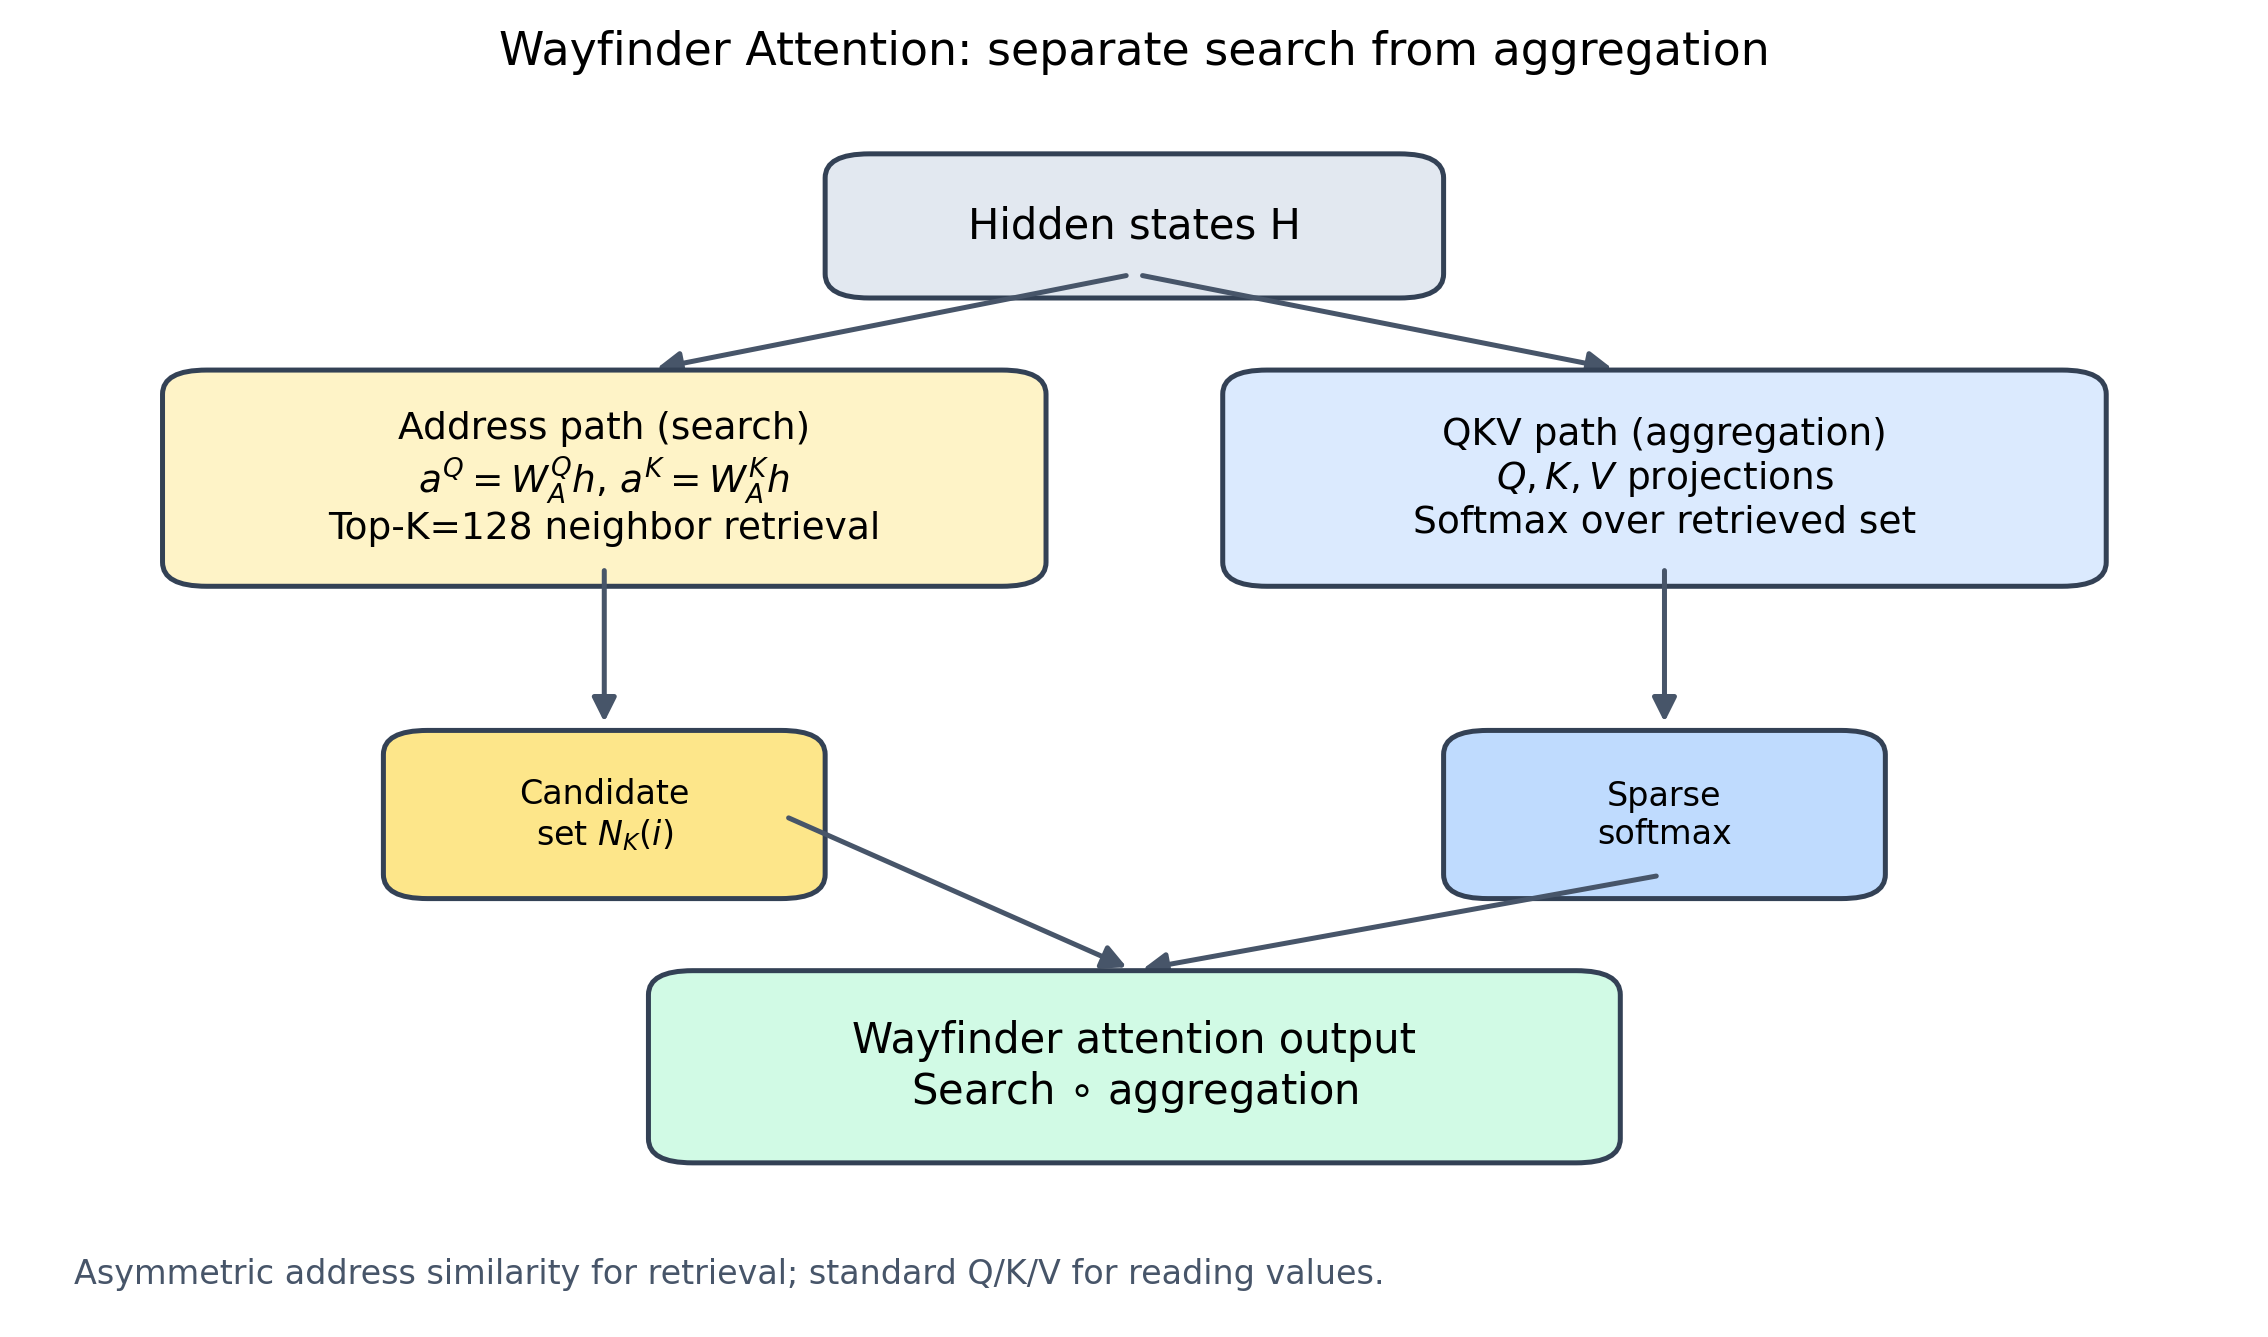
\includegraphics[width=0.96\linewidth]{fig_architecture.png}
\caption{Wayfinder Attention separates search from aggregation. The address path (search) retrieves candidate tokens; the QKV path (aggregation) computes softmax attention over the retrieved set.}
\label{fig:architecture}
\end{figure}

\subsection{Why separate addresses from query and key vectors?}

A naive sparse baseline can retrieve neighbors using the model's ordinary query and key vectors:
\begin{equation}
N_K^{\mathrm{KV}}(i)
=
\topk_{j \le i}\left(q_i^\top k_j\right).
\end{equation}
We call this the key-vector baseline. It forces the same vectors to serve indexing and softmax aggregation. Wayfinder separates these roles: dedicated address projections for search; ordinary QKV projections for aggregation. Prior learned-index sparse attention motivates this split \cite{sun2022lha,deepseek2025v32,desai2025hashattention,lou2024sparsek}; our experiments test whether it matters when the sparse forward budget is held fixed.

The address score is asymmetric:
\begin{equation}
r_{ij}^{\mathrm{asym}}
=
(W_A^Q h_i)^\top (W_A^K h_j).
\end{equation}
This matches the directed nature of causal attention: token $i$ attending to $j$ is not equivalent to $j$ attending to $i$. Asymmetric routing gave the strongest neighborhood-recall results in early index-quality experiments. RouterMLP achieved the best MNIST Recall@32 in those experiments, but our main NIAH experiments use the simpler decoupled learned-address mechanism studied here.

\section{Training Protocol}

Wayfinder Attention is trained in three phases.

\begin{figure}[H]
\centering
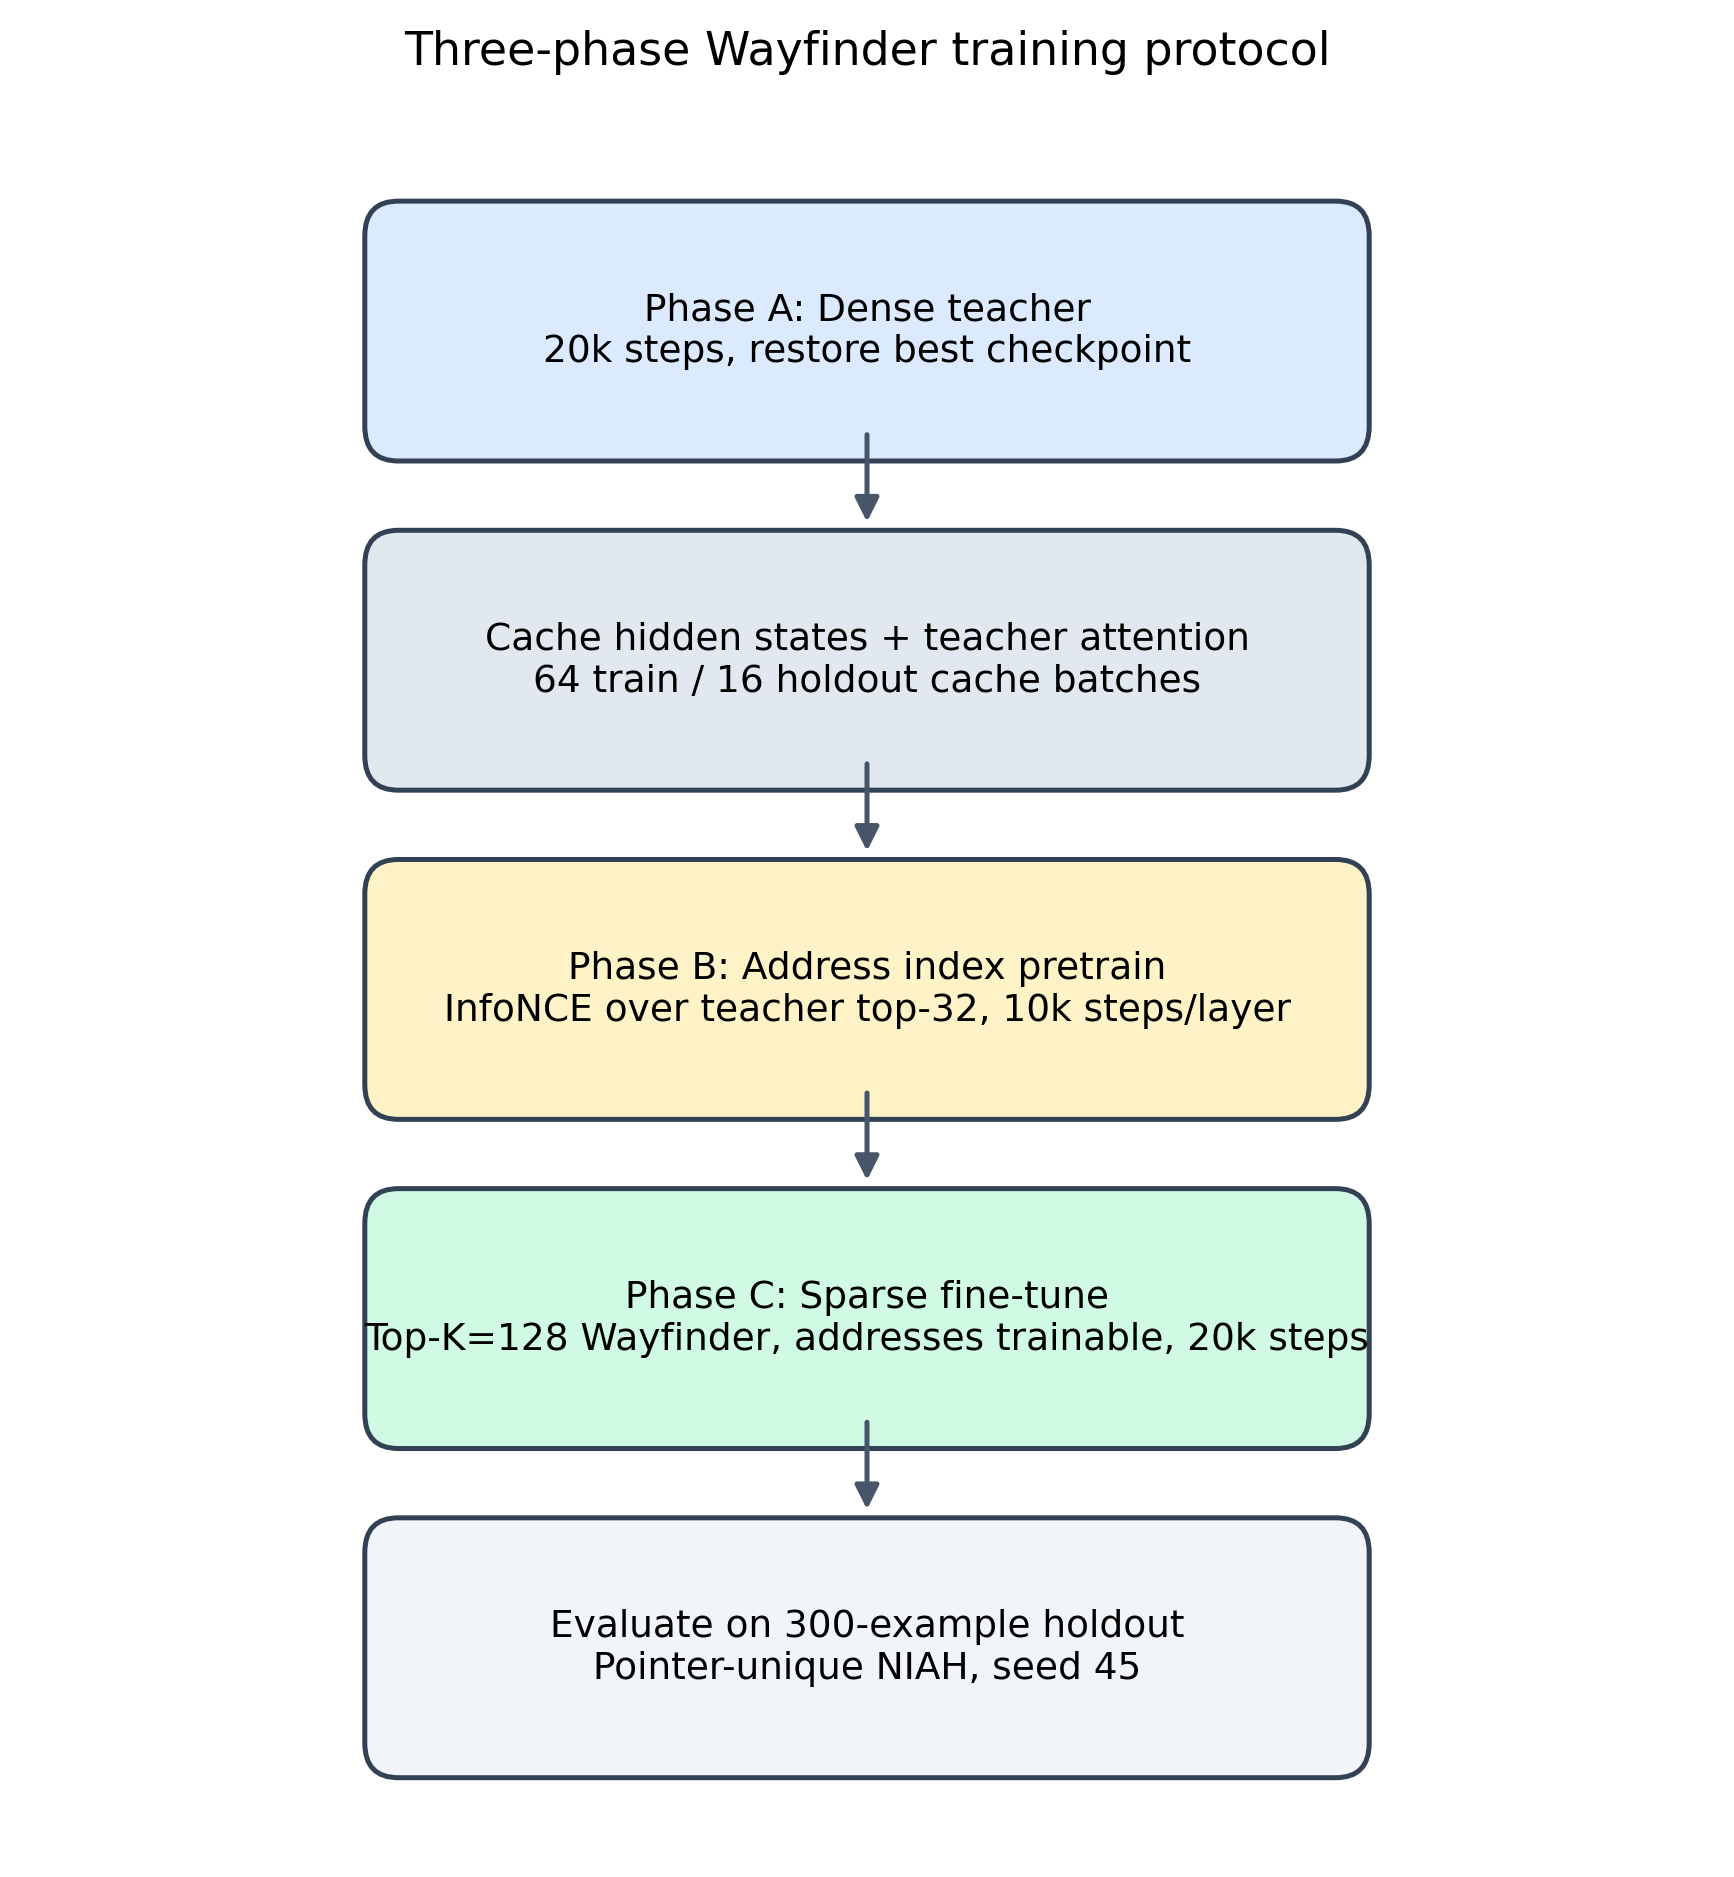
\includegraphics[width=0.92\linewidth]{fig_protocol.png}
\caption{Training recipe for the canonical experiments. Phase B initializes the address path; Phase C jointly adapts the address and QKV paths.}
\label{fig:protocol}
\end{figure}

\subsection{Phase A: Dense teacher training}

We first train a dense attention model on the task:
\begin{equation}
\theta_{\mathrm{dense}}
=
\arg\min_{\theta}
L_{\mathrm{task}}(\theta).
\end{equation}
The dense model provides both a quality reference and teacher attention neighborhoods.

\subsection{Phase B: Address-index pretraining}

We freeze the dense teacher and cache hidden states and attention maps. Address modules are trained sequentially per layer. The Phase B cache uses 64 train batches and 16 holdout batches. For each layer and query position $i$, let
\begin{equation}
P(i)
=
\topk_{32}\left(A_i^{\mathrm{teacher}}\right)
\end{equation}
denote the teacher's top-32 attended causal key positions used as InfoNCE positives. Phase B supervises address ranking with teacher top-32 neighborhoods at temperature $\tau=0.07$. This differs from the Phase C sparse forward pass, which retrieves $K=128$ candidates.

We train only the address projections using multi-positive InfoNCE:
\begin{equation}
L_i^{\mathrm{addr}}
=
-
\log
\frac{
\sum_{j \in P(i)} \exp(r_{ij}/\tau)
}{
\sum_{j \le i} \exp(r_{ij}/\tau)
}.
\end{equation}
The full address loss averages over positions and layers:
\begin{equation}
L_{\mathrm{addr}}
=
\frac{1}{|\mathcal{L}|T}
\sum_{\ell \in \mathcal{L}}
\sum_{i=1}^{T}
L_{i,\ell}^{\mathrm{addr}} .
\end{equation}

This objective trains a retrieval geometry. It does not attempt to reproduce every attention probability.

\subsection{Phase C: Sparse fine-tuning}

Finally, we replace dense attention with top-$K$ Wayfinder Attention and fine-tune on the original task:
\begin{equation}
\theta_{\mathrm{sparse}}
=
\arg\min_{\theta}
L_{\mathrm{task}}\left(\theta; N_K(i)\right).
\end{equation}
This adapts the model to softmax aggregation over retrieved candidates rather than the full causal prefix. Address projections remain trainable during Phase C (\texttt{freeze\_addresses=false}). Phase B initializes the address path; Phase C jointly adapts address, QKV, feedforward, and other trainable parameters under the sparse forward path.

\subsection{Algorithm summary}

\begin{figure}[H]
\centering
\fbox{%
\begin{minipage}{0.92\linewidth}
\textbf{Algorithm 1: Three-phase Wayfinder training}\\[0.35em]
\begin{enumerate}
    \item Train dense teacher on the retrieval task for 20k steps and restore the best checkpoint.
    \item Run the teacher to cache hidden states and dense attention neighborhoods.
    \item For each transformer layer, train asymmetric address projections using multi-positive InfoNCE over teacher top-32 neighborhoods.
    \item Replace dense attention with Wayfinder sparse attention using forward top-$K=128$.
    \item Initialize from the dense teacher and Phase B addresses; fine-tune on the original answer-only task objective with addresses left trainable.
\end{enumerate}
\end{minipage}}
\caption{Training summary. This recipe is part of the method; from-scratch long-context sparse training without these phases collapsed in excluded runs.}
\label{fig:algorithm}
\end{figure}

\subsection{Forward-pass $K$ versus diagnostic Recall@K}

Unless otherwise noted, the sparse forward pass uses $K=128$ for both Wayfinder and the key-vector baseline. Phase B InfoNCE uses the teacher's top-32 neighbors as positives---a smaller supervision set than the Phase C retrieval budget. Index diagnostics therefore mix $K$ values: Wayfinder quality is reported as teacher-neighborhood Recall@32 after Phase B; key-vector geometry as Recall@128 on the same holdout cache. We do not treat Recall@K as pass/fail because teacher-neighbor recall and downstream accuracy can diverge even when both sparse variants share forward $K=128$.

\section{Why InfoNCE Instead of MSE?}

A natural alternative is to regress the full teacher attention matrix:
\begin{equation}
L_{\mathrm{MSE}}
=
\left\|
A_Q A_K^\top - A^{\mathrm{teacher}}
\right\|_2^2 .
\end{equation}
This failed in early MNIST routing-recall experiments, achieving only 15.4\% Recall@32, below the random baseline of approximately 17\% on the MNIST teacher-cache setup with $T=784$.

The reason is objective mismatch. Sparse retrieval needs important neighbors to rank inside the top-$K$ set, not every low-mass entry to be numerically accurate. At long sequence length, most causal attention entries are near-zero tails, so full-matrix MSE spends gradient budget on unimportant negatives.

InfoNCE directly optimizes a ranking problem:
\begin{equation}
\topk(R)
\approx
\topk(A^{\mathrm{teacher}}),
\end{equation}
where $R$ is the address-score matrix. Negatives enter through the denominator:
\begin{equation}
\sum_{j \le i} \exp(r_{ij}/\tau).
\end{equation}
Hard negatives receive large gradients when their softmax probability is high; easy negatives receive little. This matches the inference-time need for top-$K$ nearest-neighbor retrieval.

\paragraph{Tensor shapes.}
For $T=2048$, $d_{\mathrm{model}}=256$, and $d_A=32$:
\begin{align}
H &\in \mathbb{R}^{2048 \times 256}, \\
A_Q &= H W_A^Q \in \mathbb{R}^{2048 \times 32}, \\
A_K &= H W_A^K \in \mathbb{R}^{2048 \times 32}, \\
R &= A_Q A_K^\top \in \mathbb{R}^{2048 \times 2048}.
\end{align}

\section{Complexity and Implementation}

\subsection{Causal exact top-$K$ retrieval}

The address path solves a constrained vector search problem. For each query position $i \in \{1,\ldots,T\}$, Wayfinder retrieves
\begin{equation}
N_K(i)=\topk_{j \le i}\; (a_i^Q)^\top a_j^K ,
\end{equation}
i.e., the top-$K$ previous tokens under cosine similarity after L2-normalizing address vectors. This is \emph{exact} maximum inner-product search (MIPS) over the causal prefix $\{1,\ldots,i\}$, not an approximate nearest-neighbor (ANN) query of the kind used in large-scale RAG systems with HNSW or IVF indexes. External RAG search targets a static corpus of millions of documents with sublinear query time and controllable recall loss; Wayfinder search targets the $i$ preceding tokens in the \emph{same forward pass}, with causality built in and no separate index build step.

\paragraph{Relation to RAG-style search.}
The RAG analogy is structural: retrieve a small candidate set, then read/aggregate. Our implementation does \emph{not} use ANN graph traversal or inverted-file quantization; it uses IO-efficient \emph{exact} top-$K$ kernels over low-dimensional addresses ($d_A=32$). Optional FAISS flat/HNSW backends were unsuitable in-layer: our prototype rebuilds indexes per forward, copies GPU tensors to CPU, and post-filters causally in Python---overhead that dominated runtime versus fused GPU causal top-$K$. Reported systems benchmarks use the \texttt{fused\_causal} exact path on CUDA.

\paragraph{Compute and memory.}
Let $B$ denote batch size. Naive retrieval materializes a full score matrix $S \in \mathbb{R}^{B \times T \times T}$ with $S_{b,i,j}=(a_i^Q)^\top a_j^K$, applies a causal mask, and runs top-$K$ per row. This costs $\Theta(BT^2 d_A)$ arithmetic and $\Theta(BT^2)$ high-bandwidth memory (HBM) traffic for storing $S$---the same scaling bottleneck that motivates FlashAttention for dense attention.

Our \texttt{fused\_causal} retriever avoids materializing $S$. It processes query rows in blocks of size $B_m$ and scores only against keys $j \le i$ within each causal tile. Peak workspace is $\mathcal{O}(B \cdot B_m \cdot T)$ score entries per block rather than $\mathcal{O}(BT^2)$. A streaming variant maintains a running width-$(K\!+\!B_j)$ top-$K$ heap while multiplying query blocks against key tiles of width $B_j$, merging candidates without ever holding an $(T \times T)$ buffer. Total address-search arithmetic remains $\Theta(BT^2 d_A)$ for exact causal MIPS, but HBM traffic drops sharply because scores are produced, masked, reduced to top-$K$, and discarded tile-by-tile---the same memory-bandwidth logic that makes fused attention kernels faster than unfused matmul+softmax at long context. Figure~\ref{fig:retrieval-tiling} summarizes this distinction.

\begin{figure}[H]
\centering
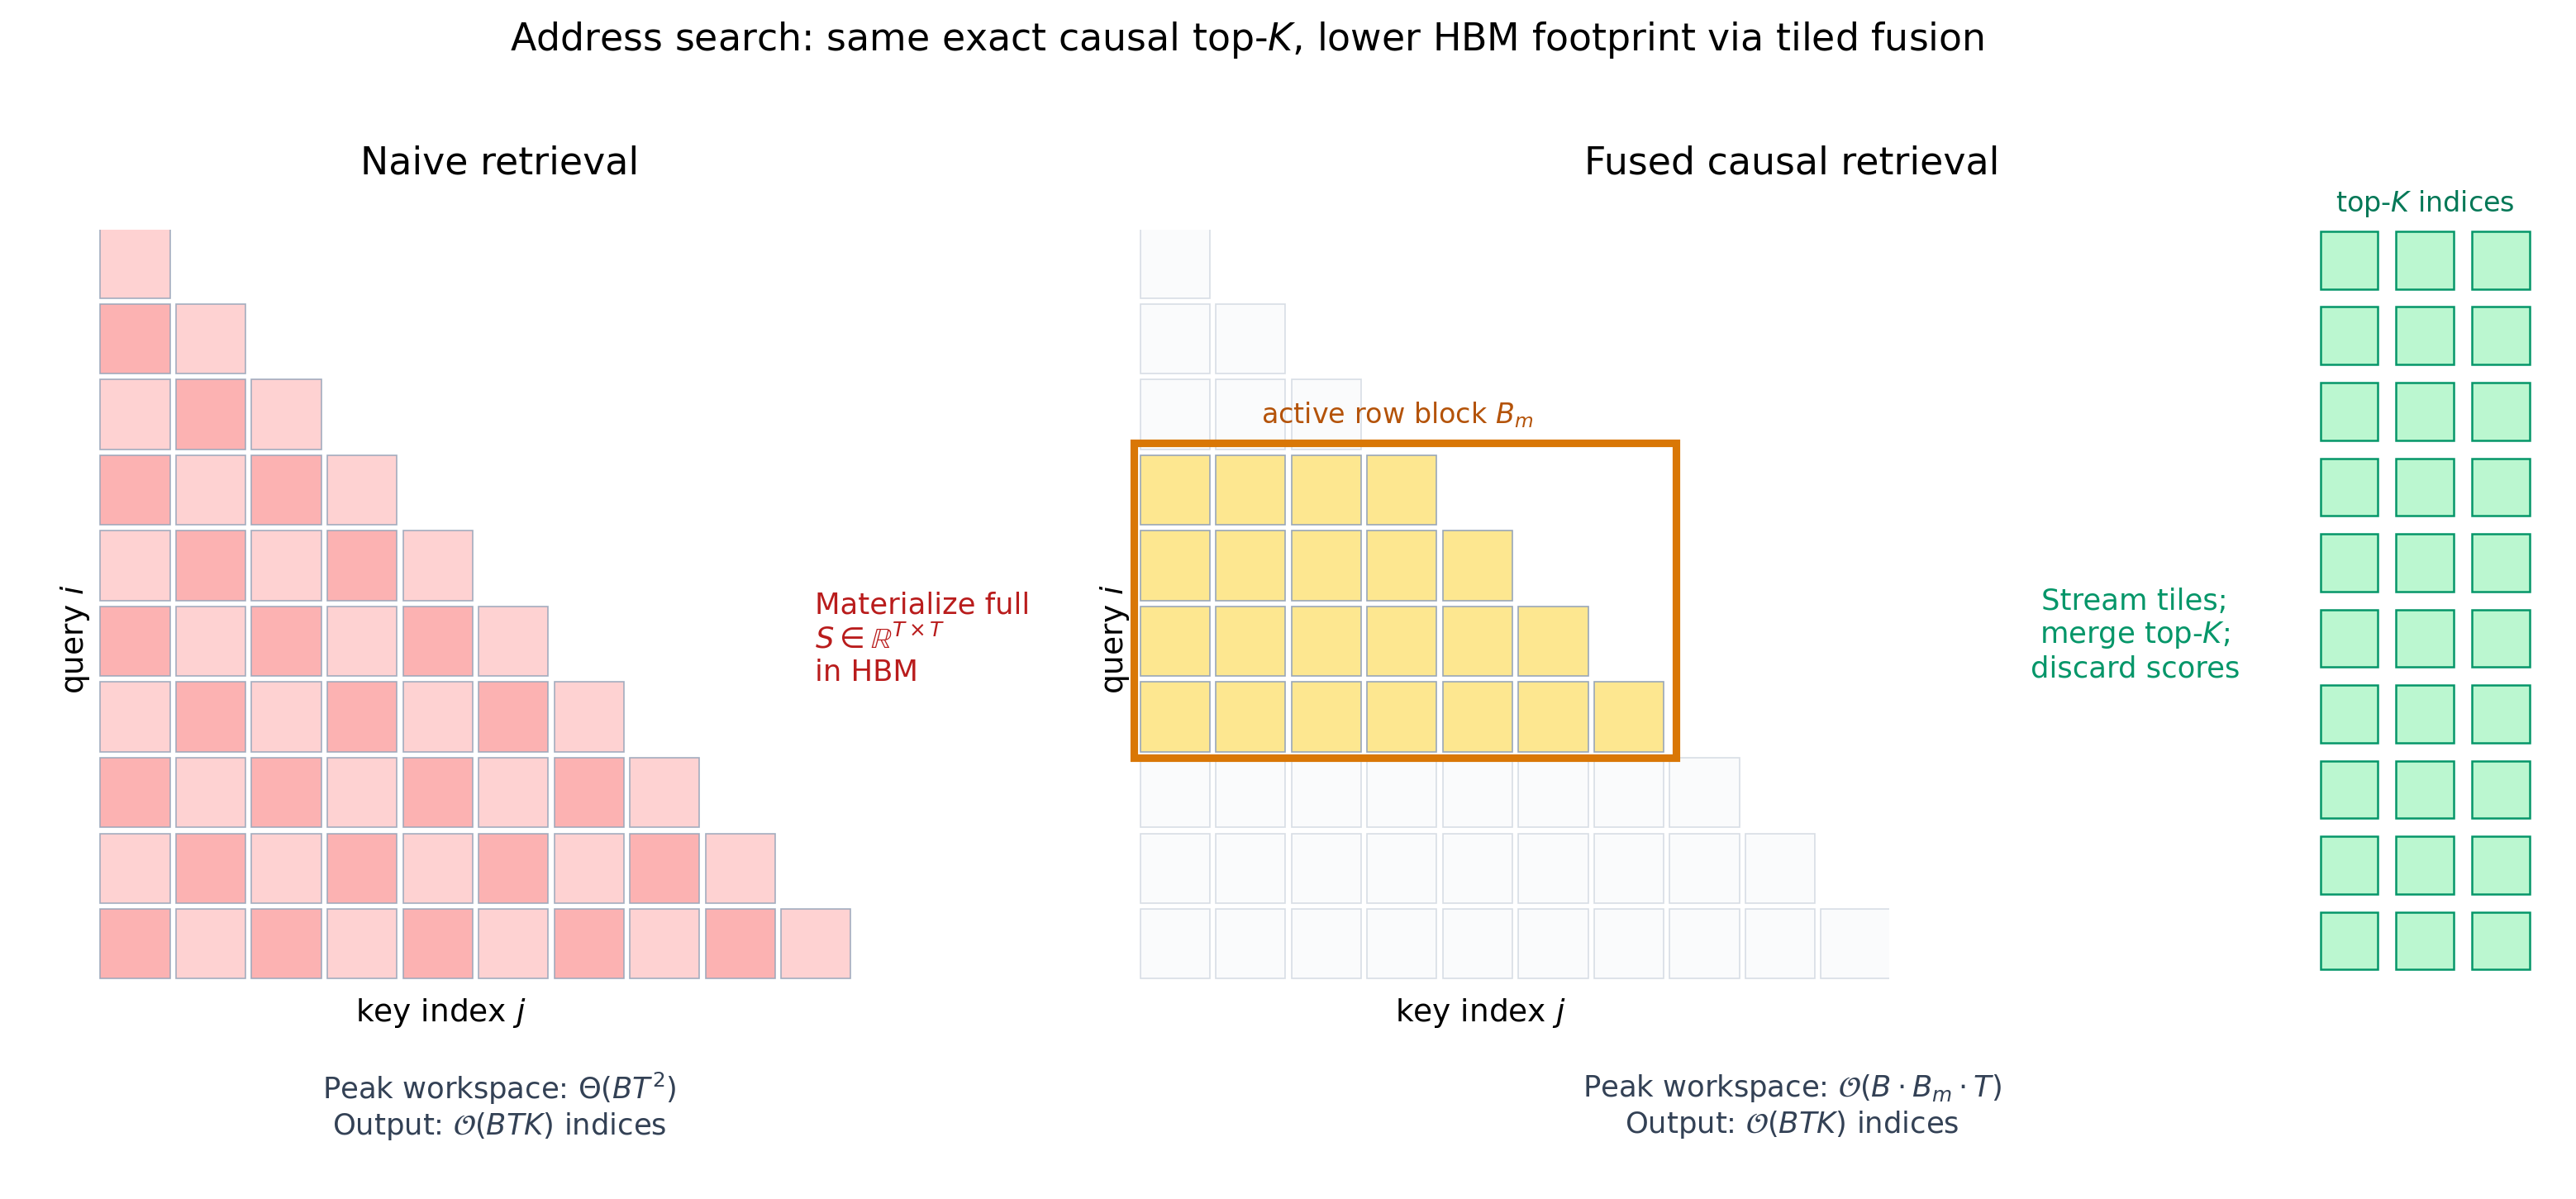
\includegraphics[width=0.98\linewidth]{fig_retrieval_tiling.png}
\caption{Naive versus fused causal address retrieval. Both paths compute exact causal top-$K$ MIPS and emit $\mathcal{O}(BTK)$ indices. \textbf{Left:} materialize the full $T \times T$ score matrix in HBM (peak workspace $\Theta(BT^2)$), then causal mask and top-$K$. \textbf{Right:} stream causal query row blocks and key tiles with running top-$K$ merge (peak workspace $\mathcal{O}(B B_m T)$). Fusion reduces peak HBM footprint without changing the retrieval objective.}
\label{fig:retrieval-tiling}
\end{figure}

\paragraph{Output and aggregation complexity.}
Retrieval outputs only $\mathcal{O}(BTK)$ integer indices (and optionally top-$K$ scores). The QKV path then computes head-wise softmax attention over those $K$ neighbors:
\begin{equation}
\mathrm{QKV\ work}=\mathcal{O}(B H T K d_h),
\end{equation}
where $H$ is the number of heads and $d_h$ the head dimension. Dense causal attention costs $\mathcal{O}(B H T^2 d_h)$ for the analogous combined score-and-aggregate path. Wayfinder instead pays $\Theta(B T^2 d_A)$ for exact address search plus $\mathcal{O}(B H T K d_h)$ for sparse QKV readout. When $K \ll T$ and $d_A \ll d_h$, the dominant $T^2 d_h$ dense-attention term is replaced by $T K d_h$ on the readout path; address search adds a smaller-coefficient $T^2 d_A$ term rather than sublinear query time.

\subsection{Sparse attention edges and speedup}

Dense attention computes $O(T^2)$ candidate \emph{attention} edges per layer. After retrieval, Wayfinder computes softmax attention over only $K$ neighbors per token:
\begin{equation}
\mathrm{Sparse\ edges} = O(TK).
\end{equation}
The ideal \emph{attention-edge} reduction from dense to sparse readout is
\begin{equation}
\frac{T^2}{TK} = \frac{T}{K}.
\end{equation}
For $T=8192$ and $K=128$, this is a 64-fold reduction in QKV edges; for $K=32$ it would be 256-fold. Our main experiments use $K=128$ at inference. Address search adds exact causal top-$K$ with FLOPs $\Theta(T^2 d_A)$ but fused implementation avoids a full $T \times T$ score matrix; wall-clock crossover depends on $\mathcal{O}(T K d_h)$ QKV savings, $d_A \ll d_h$, and kernel fusion, not sublinear vector search or edge count alone.

This edge-count argument does not imply wall-clock speedup. Dense attention uses highly optimized fused kernels; sparse attention adds retrieval, gather, masking, and small softmax ops. In our prototype, dense FlashAttention is faster at short lengths; Wayfinder becomes faster at longer lengths.

\paragraph{Prototype GPU kernels.}
Making sparse Wayfinder attention practical at long context required custom kernels, not only a topology change. Naive sparse attention materializes or streams an $O(T^2)$ address score matrix; our prototype avoids that. The \emph{address path} uses \texttt{fused\_causal} top-$K$ retrieval: row-blocked triangular scoring over L2-normalized addresses, with optional Triton heap kernels, producing causal neighbor indices without a full score matrix in HBM. The \emph{QKV path} gathers over those indices and applies softmax in a fused sparse pipeline (\texttt{use\_fused\_sparse=true}) with batched GPU kernels and head-parallel Triton paths. Legacy FAISS hooks remain for comparison but were too slow in our dynamic causal setting and are not used in the main experiments or systems benchmarks. These are prototype implementations, not production-tuned primitives; we report latency and memory as engineering measurements rather than claiming kernel parity with FlashAttention.

\paragraph{Kernel status.}
The systems numbers should be interpreted as prototype measurements of the fused retrieval + sparse aggregation stack, benchmarked against dense Flash scaled dot-product attention under the same small model configuration. Remaining gaps include end-to-end fusion of retrieval with QKV aggregation, broader dtype and block-size tuning, and head/batch scaling studies.

\section{Experimental Setup}

\subsection{Synthetic pointer retrieval task}

We evaluate on a controlled needle-in-a-haystack benchmark: random filler, one unique key--value binding, and a suffix query. The target is the value for the queried key. The task isolates long-range retrieval without natural language modeling.

Needle depths are 10\%, 25\%, 50\%, 75\%, and 90\% of context. The holdout uses 300 examples with a disjoint holdout seed. The main setting has zero decoys. Training uses answer-only supervision (weight 8.0); evaluation reports exact match on the answer token.

\subsection{Canonical model and training setup}

Table~\ref{tab:setup} summarizes the experimental configuration.

\begin{table}[H]
\caption{Canonical proof-cell configuration.}
\centering
\small
\begin{tabular}{p{0.32\linewidth}p{0.58\linewidth}}
\toprule
Setting & Value \\
\midrule
Task & Pointer-unique NIAH \\
Sequence lengths & 2048 and 4096 (trained quality) \\
Length curriculum & 4096 initializes from the 2048 checkpoint \\
Needle depths & 10\%, 25\%, 50\%, 75\%, 90\% \\
Decoys & 0 \\
Training objective & answer-only, answer loss weight 8.0 \\
Model & 4-layer causal transformer \\
Hidden dimension & 256 \\
Attention heads & 4 \\
Feedforward dimension & 1024 \\
Vocabulary size & 257 \\
Address dimension $d_A$ & 32 (\texttt{k32} suffix; not forward $K$) \\
Sparse forward top-$K$ & 128 (Wayfinder and key-vector) \\
Phase B InfoNCE positives & teacher top-32 neighbors \\
Phase A steps & 20,000, restore-best checkpoint \\
Phase B steps & 10,000 per layer unless swept \\
Phase B cache & 64 train batches / 16 holdout batches \\
Phase B temperature & $\tau=0.07$ \\
Phase C steps & 20,000, addresses trainable \\
Batch size & 4 for training; 1 for systems benchmark \\
Learning rate & $3 \times 10^{-4}$ \\
Warmup & 500 steps \\
Train seed & 45 \\
Holdout seed & 1000042 \\
Holdout size & 300 examples \\
Hardware & RTX 5090, WSL \\
Reproducibility & Canonical results: \texttt{experiments/Experiment\_7/learned\_address\_proof\_cell/proof\_cell\_full/}; figure script: \texttt{scripts/generate\_wayfinder\_paper\_figures.py} \\
Code mapping & \texttt{learned\_address\_k32} (historical label: $d_A{=}32$, not forward $K$); class \texttt{LearnedAddressSparseAttention} \\
\bottomrule
\end{tabular}
\label{tab:setup}
\end{table}

\vspace*{\dimexpr-\intextsep\relax}
\begin{mainresultstight}
\section{Main Results}
\subsection{Baseline fairness}
Table~\ref{tab:fairness} summarizes baseline training. Wayfinder, key-vector sparse attention, and local-window attention initialize from the same dense teacher. Linear attention gets the same 20k-step task budget as the dense teacher but trains from scratch with linear attention---no dense Flash init and no Phase B/C. In the full run, linear attention stays near chance for many steps before reaching 100\% late in training.

{\centering
\captionsetup{type=table}
\captionof{table}{Baseline training protocol ($T{=}2048$ main experiments).}
\label{tab:fairness}
\small
\resizebox{\linewidth}{!}{%
\begin{tabular}{lcccc}
\toprule
Method & Task training & Dense teacher path & Phase B index & Phase C sparse \\
\midrule
Dense FlashAttention & Yes, 20k & Yes & No & No \\
Wayfinder Attention & Yes, 20k + 20k & Yes & Yes & Yes \\
Key-vector top-$K$ & Yes, 20k + 20k & Yes & No & Yes \\
Local $W=64/256$ & Yes, 20k + 20k & Yes & No & Yes \\
Linear attention & Yes, 20k & No & No & No \\
\bottomrule
\end{tabular}%
}
\par}

\subsection{Proof cell at sequence length 2048}
Table~\ref{tab:proof-cell} shows results at $T{=}2048$. Wayfinder matches dense attention and substantially outperforms key-vector and local-window sparse baselines.

{\centering
\captionsetup{type=table}
\captionof{table}{Canonical proof cell at sequence length 2048, 0 decoys, 4-layer model, train seed 45, holdout seed 1000042, 300-example holdout.}
\label{tab:proof-cell}
\small
\begin{tabular}{lcccccc}
\toprule
Method & Overall & 10\% & 25\% & 50\% & 75\% & 90\% \\
\midrule
Dense FlashAttention & 100.0 & 100.0 & 100.0 & 100.0 & 100.0 & 100.0 \\
Wayfinder Attention & 100.0 & 100.0 & 100.0 & 100.0 & 100.0 & 100.0 \\
Key-vector top-$K$ & 81.3 & 86.7 & 91.7 & 100.0 & 55.0 & 73.3 \\
Local window, $W=256$ & 36.3 & 13.3 & 13.3 & 5.0 & 50.0 & 100.0 \\
Local window, $W=64$ & 12.3 & 13.3 & 11.7 & 8.3 & 10.0 & 18.3 \\
Linear attention & 100.0 & 100.0 & 100.0 & 100.0 & 100.0 & 100.0 \\
\bottomrule
\end{tabular}
\par}

Wayfinder improves over key-vector sparse attention by 18.7 percentage points and over local-window $W=64$ by 87.7. The most informative key-vector failure is at 75\% depth (55.0\% vs.\ 100.0\% for Wayfinder and dense). Local $W=256$ succeeds at 90\% depth because the needle falls in the trailing window but fails at earlier depths.
\end{mainresultstight}

\begin{figure}[H]
\centering
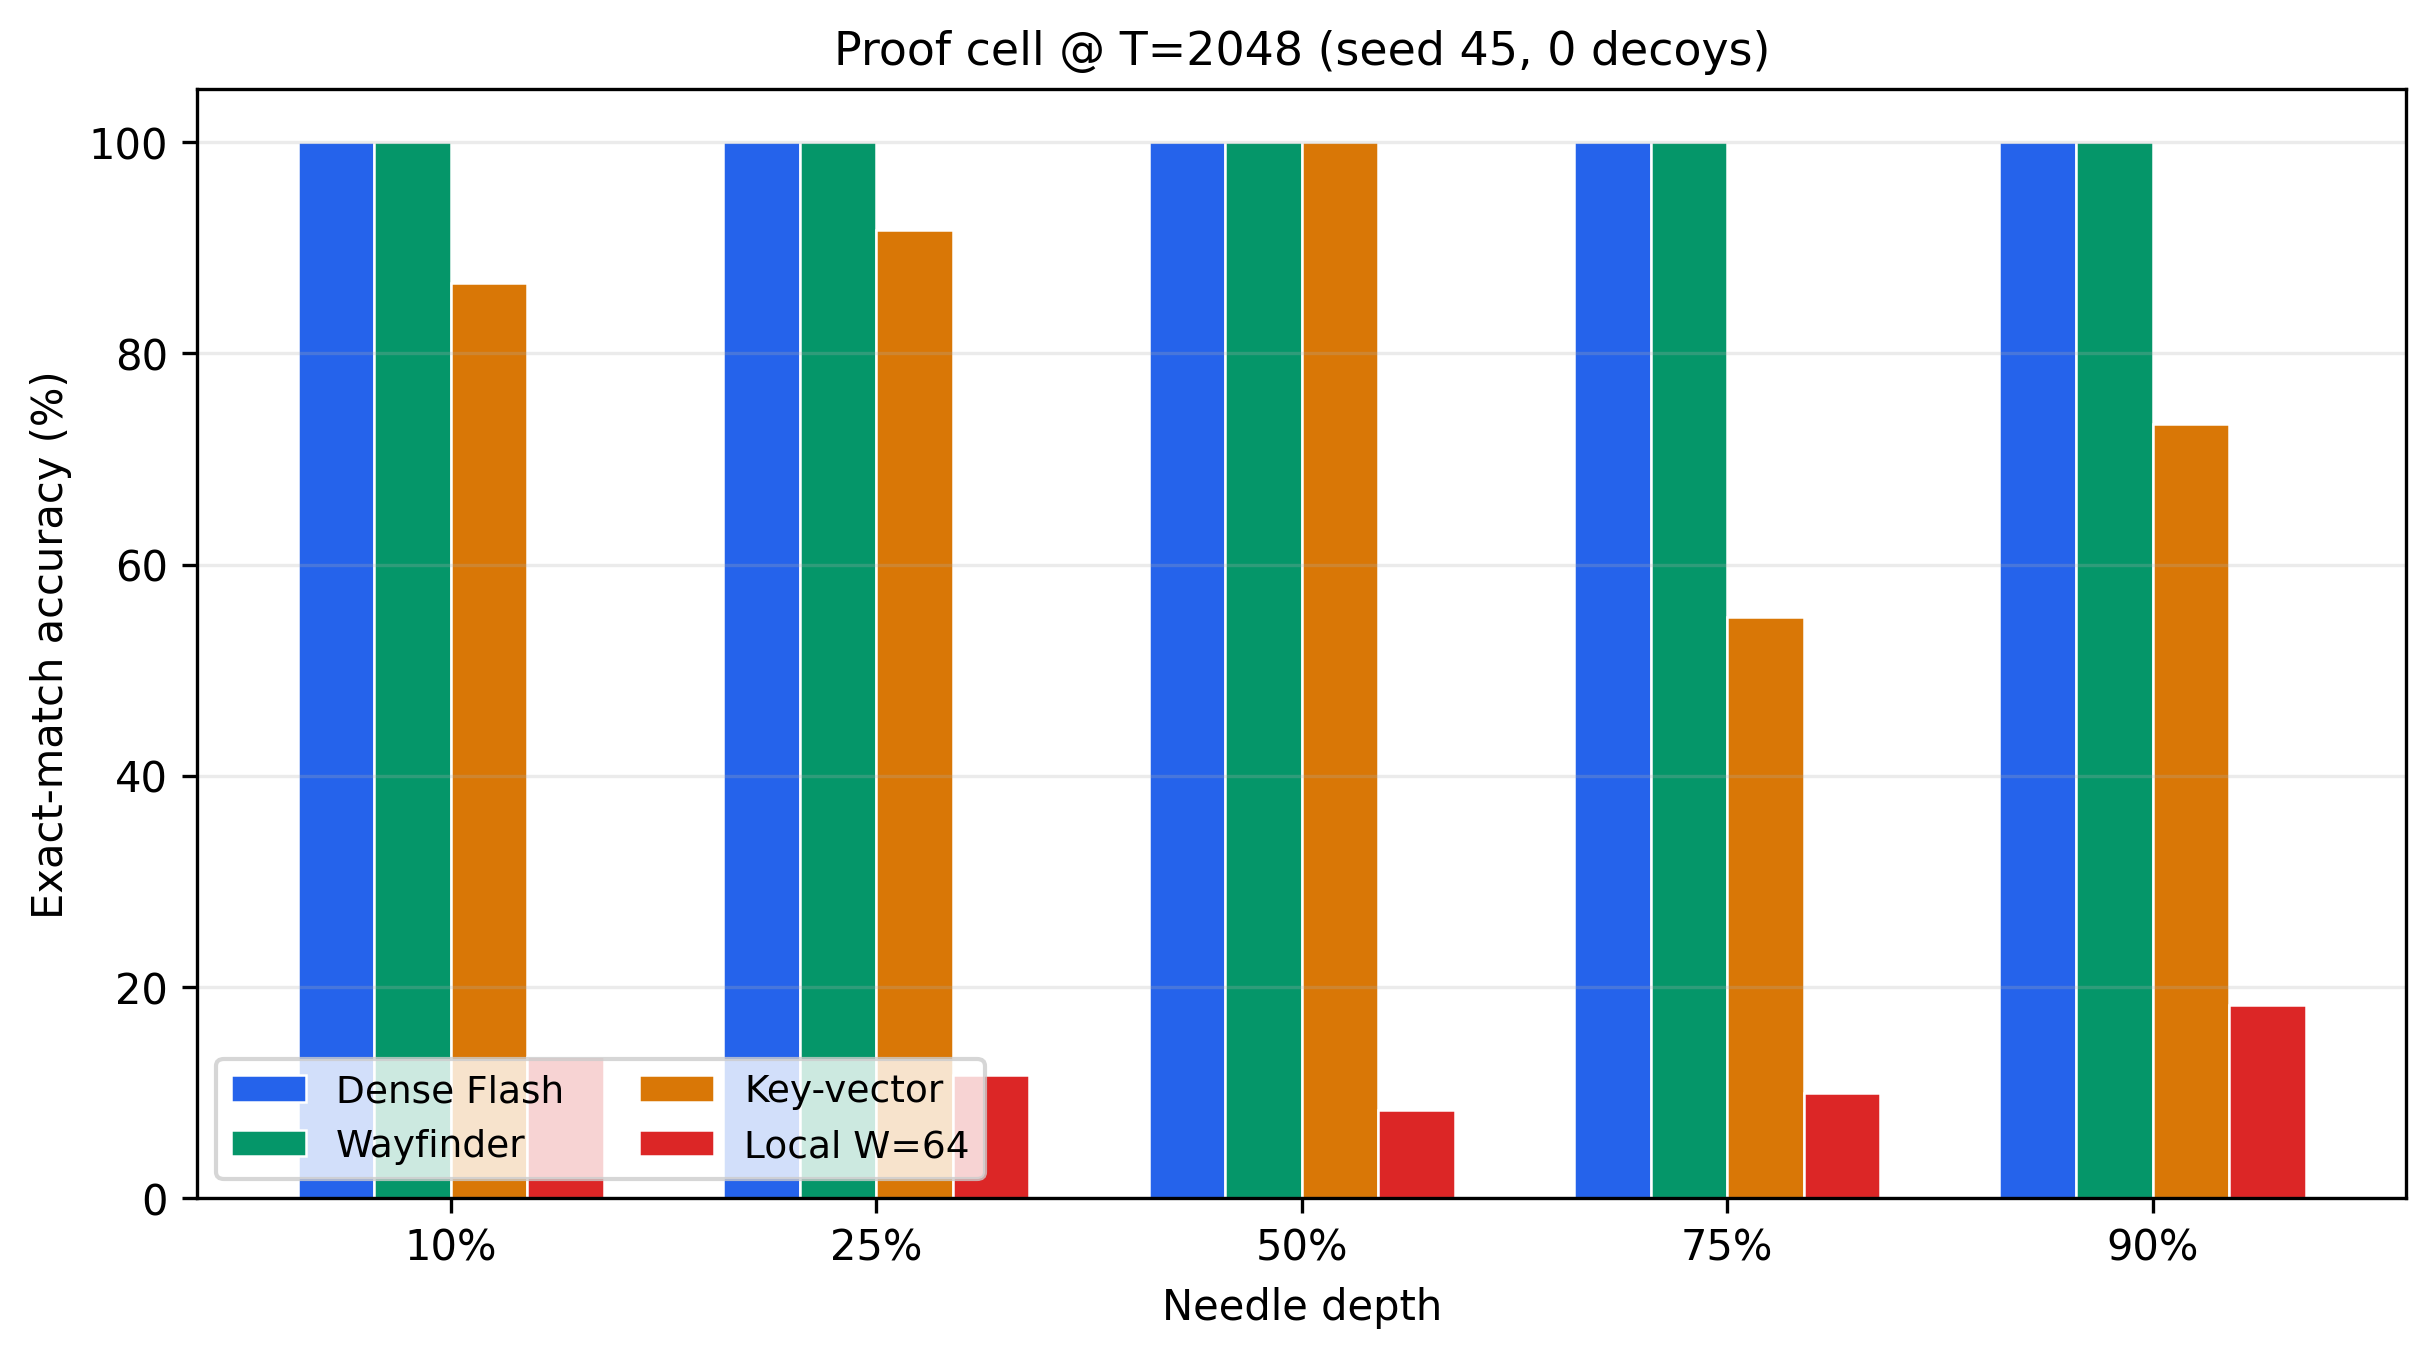
\includegraphics[width=0.95\linewidth]{fig_depth_bars.png}
\caption{Depth-stratified proof-cell accuracy at sequence length 2048. Key-vector and local-window failures are depth-dependent, while dense, Wayfinder, and linear attention solve the easy zero-decoy task.}
\label{fig:depth-bars}
\end{figure}

\subsection{Length curriculum}

Table~\ref{tab:curriculum} shows length-curriculum results through $T{=}4096$; the 4096 run initializes from the 2048 checkpoint. Recall@32 here comes from the \texttt{curriculum\_full} orchestrator and can differ from the standalone 2048 run (59.3\% in Table~\ref{tab:index-diagnostics}); Phase B recall is diagnostic, not the training objective, and both runs reach 100\% after Phase C.

\begin{table}[H]
\caption{Length curriculum under our training recipe (orchestrator \texttt{curriculum\_full}), through $T{=}4096$. Recall column: Wayfinder teacher-neighborhood Recall@32 after Phase B on each length-transfer run.}
\centering
\small
\resizebox{0.92\linewidth}{!}{%
\begin{tabular}{lccc}
\toprule
Context length & Dense FlashAttention & Wayfinder Attention & Wayfinder Recall@32 after Phase B \\
\midrule
2048 & 100.0 & 100.0 & 50.9 \\
4096 & 100.0 & 100.0 & 41.3 \\
\bottomrule
\end{tabular}%
}
\label{tab:curriculum}
\end{table}

\subsection{Phase B budget sweep}

Table~\ref{tab:bsweep} shows that downstream task accuracy at sequence length 2048 is insensitive to the number of Phase B address-training steps in the tested range.

\begin{table}[H]
\caption{Phase B address-training step sweep at sequence length 2048 (steps per layer). Recall column reports Wayfinder teacher-neighborhood Recall@32 after Phase B.}
\centering
\small
\begin{tabular}{lcc}
\toprule
Phase B steps & Phase C task accuracy & Wayfinder Recall@32 after Phase B \\
\midrule
2,000 & 100.0 & 62.5 \\
5,000 & 100.0 & 60.2 \\
10,000 & 100.0 & 59.4 \\
20,000 & 100.0 & 58.2 \\
\bottomrule
\end{tabular}
\label{tab:bsweep}
\end{table}

This suggests address pretraining need not perfectly recover the teacher attention graph---a useful sparse initialization may suffice for Phase C. Pre-Phase-C Recall@32 declines modestly with longer Phase B budgets (62.5\% to 58.2\%) without any task-accuracy drop after Phase C; we interpret this as metric mismatch. Recall@32 measures index quality before Phase C; task accuracy reflects joint address+QKV fine-tuning. InfoNCE optimizes ranking loss, not Recall@32 directly; on this easy zero-decoy cell many address initializations suffice once Phase C runs.

\begin{figure}[H]
\centering
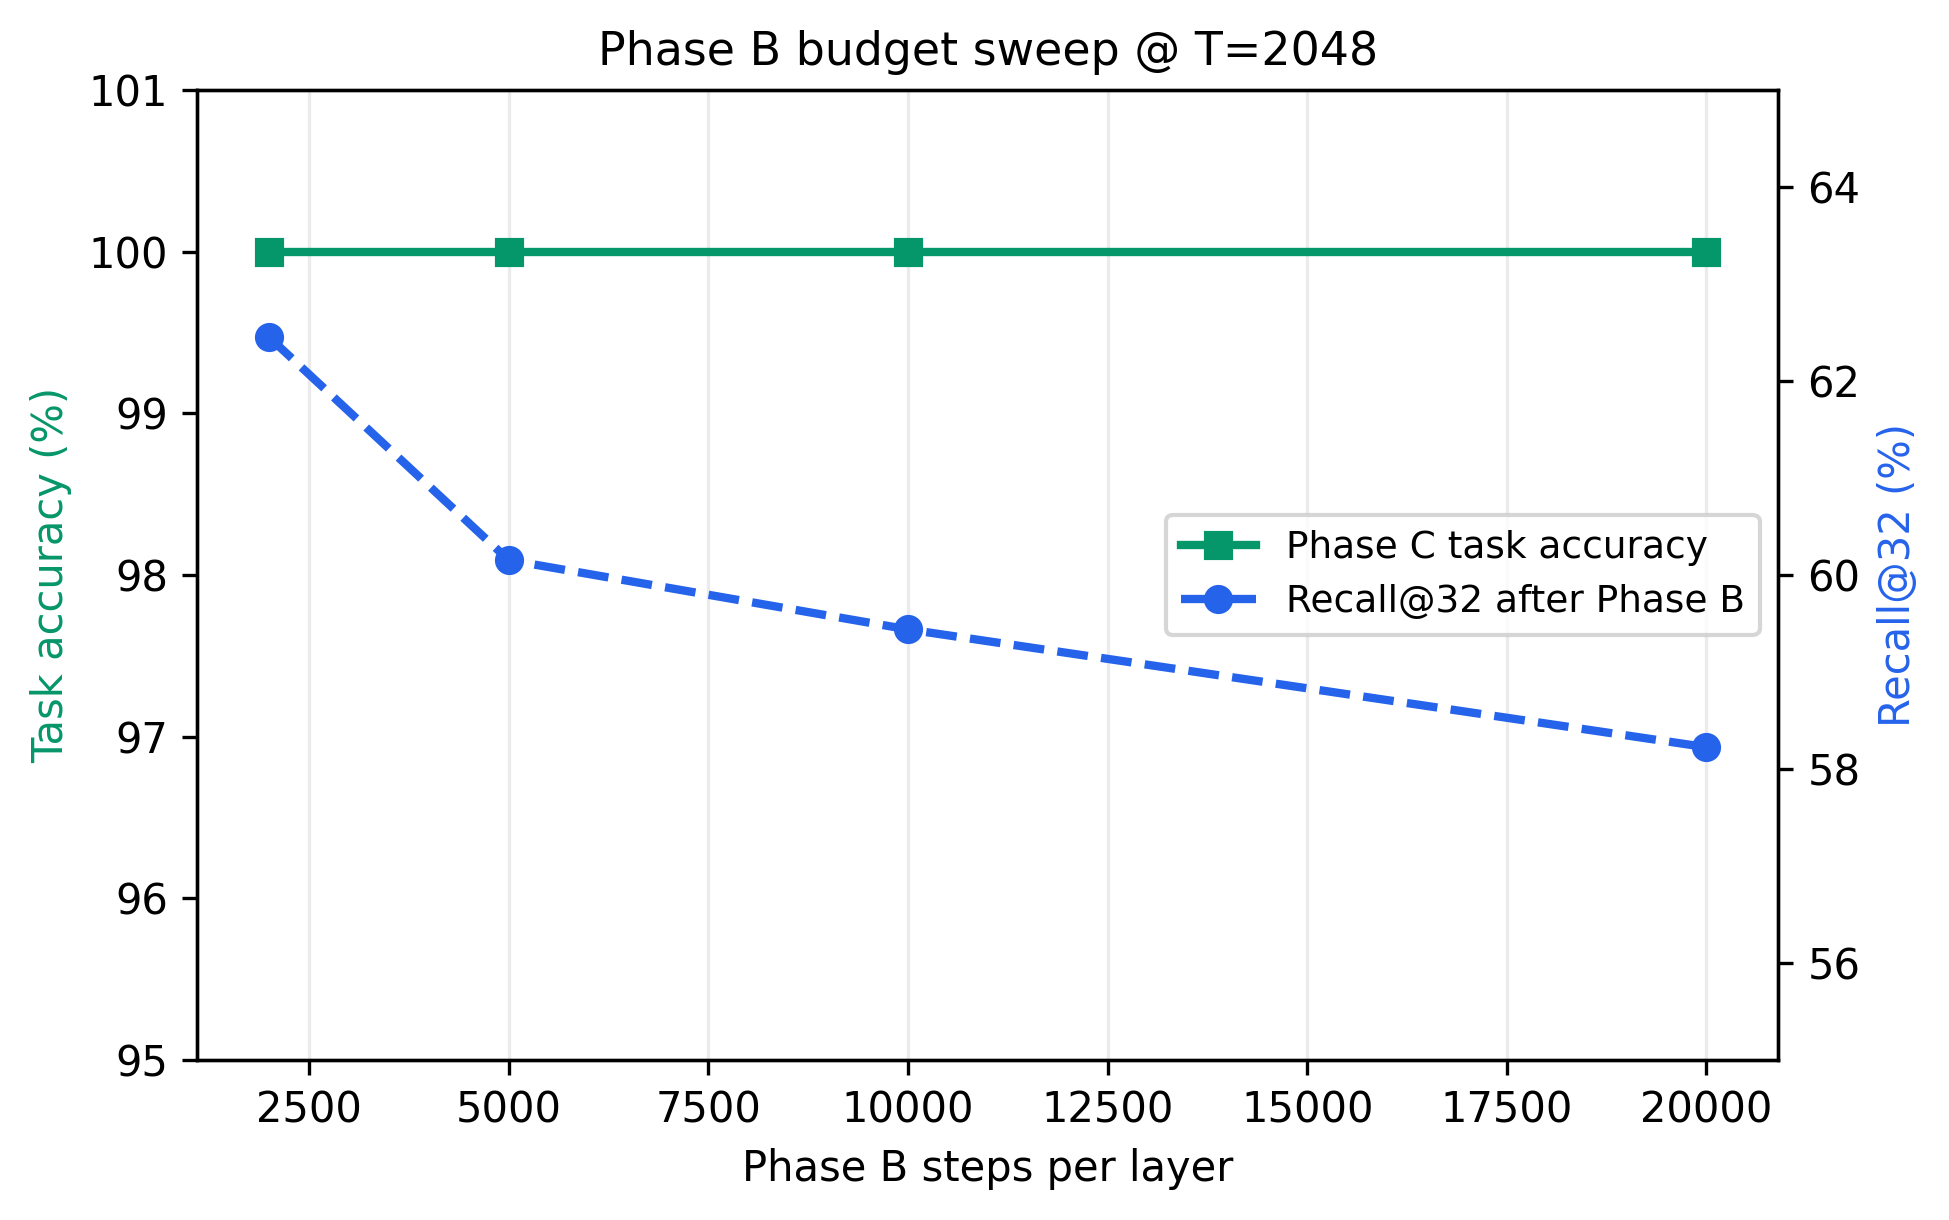
\includegraphics[width=0.78\linewidth]{fig_bsweep.png}
\caption{Phase B step sweep at sequence length 2048: downstream task accuracy stays at 100\% while Wayfinder Recall@32 after Phase B declines slightly with more address-training steps.}
\label{fig:bsweep}
\end{figure}

\subsection{Index diagnostics versus task accuracy}

Table~\ref{tab:index-diagnostics} reports a key observation, not a same-$K$ recall comparison. Key-vector geometry achieves higher Recall@128 than Wayfinder Recall@32, yet key-vector sparse attention has lower task accuracy despite both using forward top-$K=128$. Recall@K is a useful search-layer diagnostic but not a complete predictor of downstream behavior.

\begin{table}[H]
\caption{Index diagnostics versus downstream task accuracy in the 2048-token proof cell. Wayfinder recall is teacher-neighborhood Recall@32 after Phase B; key-vector recall is Recall@128 on the same holdout cache. Both sparse variants use forward top-$K=128$ at inference.}
\centering
\small
\begin{tabular}{lcc}
\toprule
Method & Teacher-neighborhood recall & Downstream task accuracy \\
\midrule
Wayfinder Attention & Recall@32: 59.3 & 100.0 \\
Key-vector top-$K$ & Recall@128: 67.1 & 81.3 \\
\bottomrule
\end{tabular}
\label{tab:index-diagnostics}
\end{table}

Higher raw teacher-neighborhood recall at a diagnostic $K$ does not guarantee better sparse attention. We attribute this to decoupling search from aggregation: the key-vector baseline uses the same geometry for finding and reading; Wayfinder uses a dedicated address space for retrieval and a separate QKV pathway for aggregation.

\section{Systems Results}

\subsection{Benchmark protocol}

Systems results use a 4-layer model (hidden 256, batch 1), forward-pass only. Dense attention uses Flash scaled dot-product attention. Wayfinder and key-vector variants use the fused causal retrieval and sparse QKV kernels in Section~6. We verified from \texttt{proof\_cell\_full/index\_checkpoints/\_address\_cache\_T2048/config.yaml} (\texttt{retrieval.method=fused\_causal}, \texttt{use\_fused\_sparse=true}) that reported rows use fused paths, not the reference full-score retrieval path. For $T>4096$, extended position embeddings apply; 8192 and 16384 rows are forward latency/memory benchmarks only, not claims about task accuracy after full training at those lengths. Dense, Wayfinder, and key-vector rows come from \texttt{systems\_benchmark.json}; linear rows from a separate session with the same harness and model config. Values are prototype measurements.

\subsection{Latency and memory}

Table~\ref{tab:systems} reports forward-pass latency and peak memory. At short context lengths, dense FlashAttention is both faster and more memory-efficient than Wayfinder in this prototype (e.g., 6.2 ms / 209 MB versus 13.8 ms / 652 MB at $T{=}2048$), reflecting retrieval and gather overhead before the QKV crossover pays off. Wayfinder becomes faster at longer context lengths. In our prototype, the latency crossover occurs between 4096 and 8192 tokens: dense is faster at 4096 tokens (7.7 ms versus 27.5 ms), while Wayfinder is faster at 8192 tokens (19.8 ms versus 27.3 ms) and 16384 tokens (38.3 ms versus 84.3 ms).

\begin{table}[H]
\caption{Forward-pass systems benchmark, 4-layer model, batch size 1, sparse forward $K=128$ for Wayfinder and key-vector. Values are latency / peak VRAM. Dense, Wayfinder, and key-vector rows are from the canonical proof-cell benchmark; linear rows are from a separate run of the same harness.}
\centering
\small
\resizebox{\linewidth}{!}{%
\begin{tabular}{lcccc}
\toprule
Length & Dense Flash & Wayfinder & Key-vector & Linear \\
\midrule
2048 & 6.2 ms / 209 MB & 13.8 ms / 652 MB & 13.5 ms / 515 MB & 11 ms / 140 MB \\
4096 & 7.7 ms / 477 MB & 27.5 ms / 664 MB & 30.2 ms / 665 MB & 7 ms / 169 MB \\
8192 & 27.3 ms / 1517 MB & 19.8 ms / 963 MB & 20.7 ms / 964 MB & 10 ms / 230 MB \\
16384 & 84.3 ms / 5614 MB & 38.3 ms / 2328 MB & 37.6 ms / 2332 MB & 18 ms / 350 MB \\
\bottomrule
\end{tabular}%
}
\label{tab:systems}
\end{table}

\begin{figure}[H]
\centering
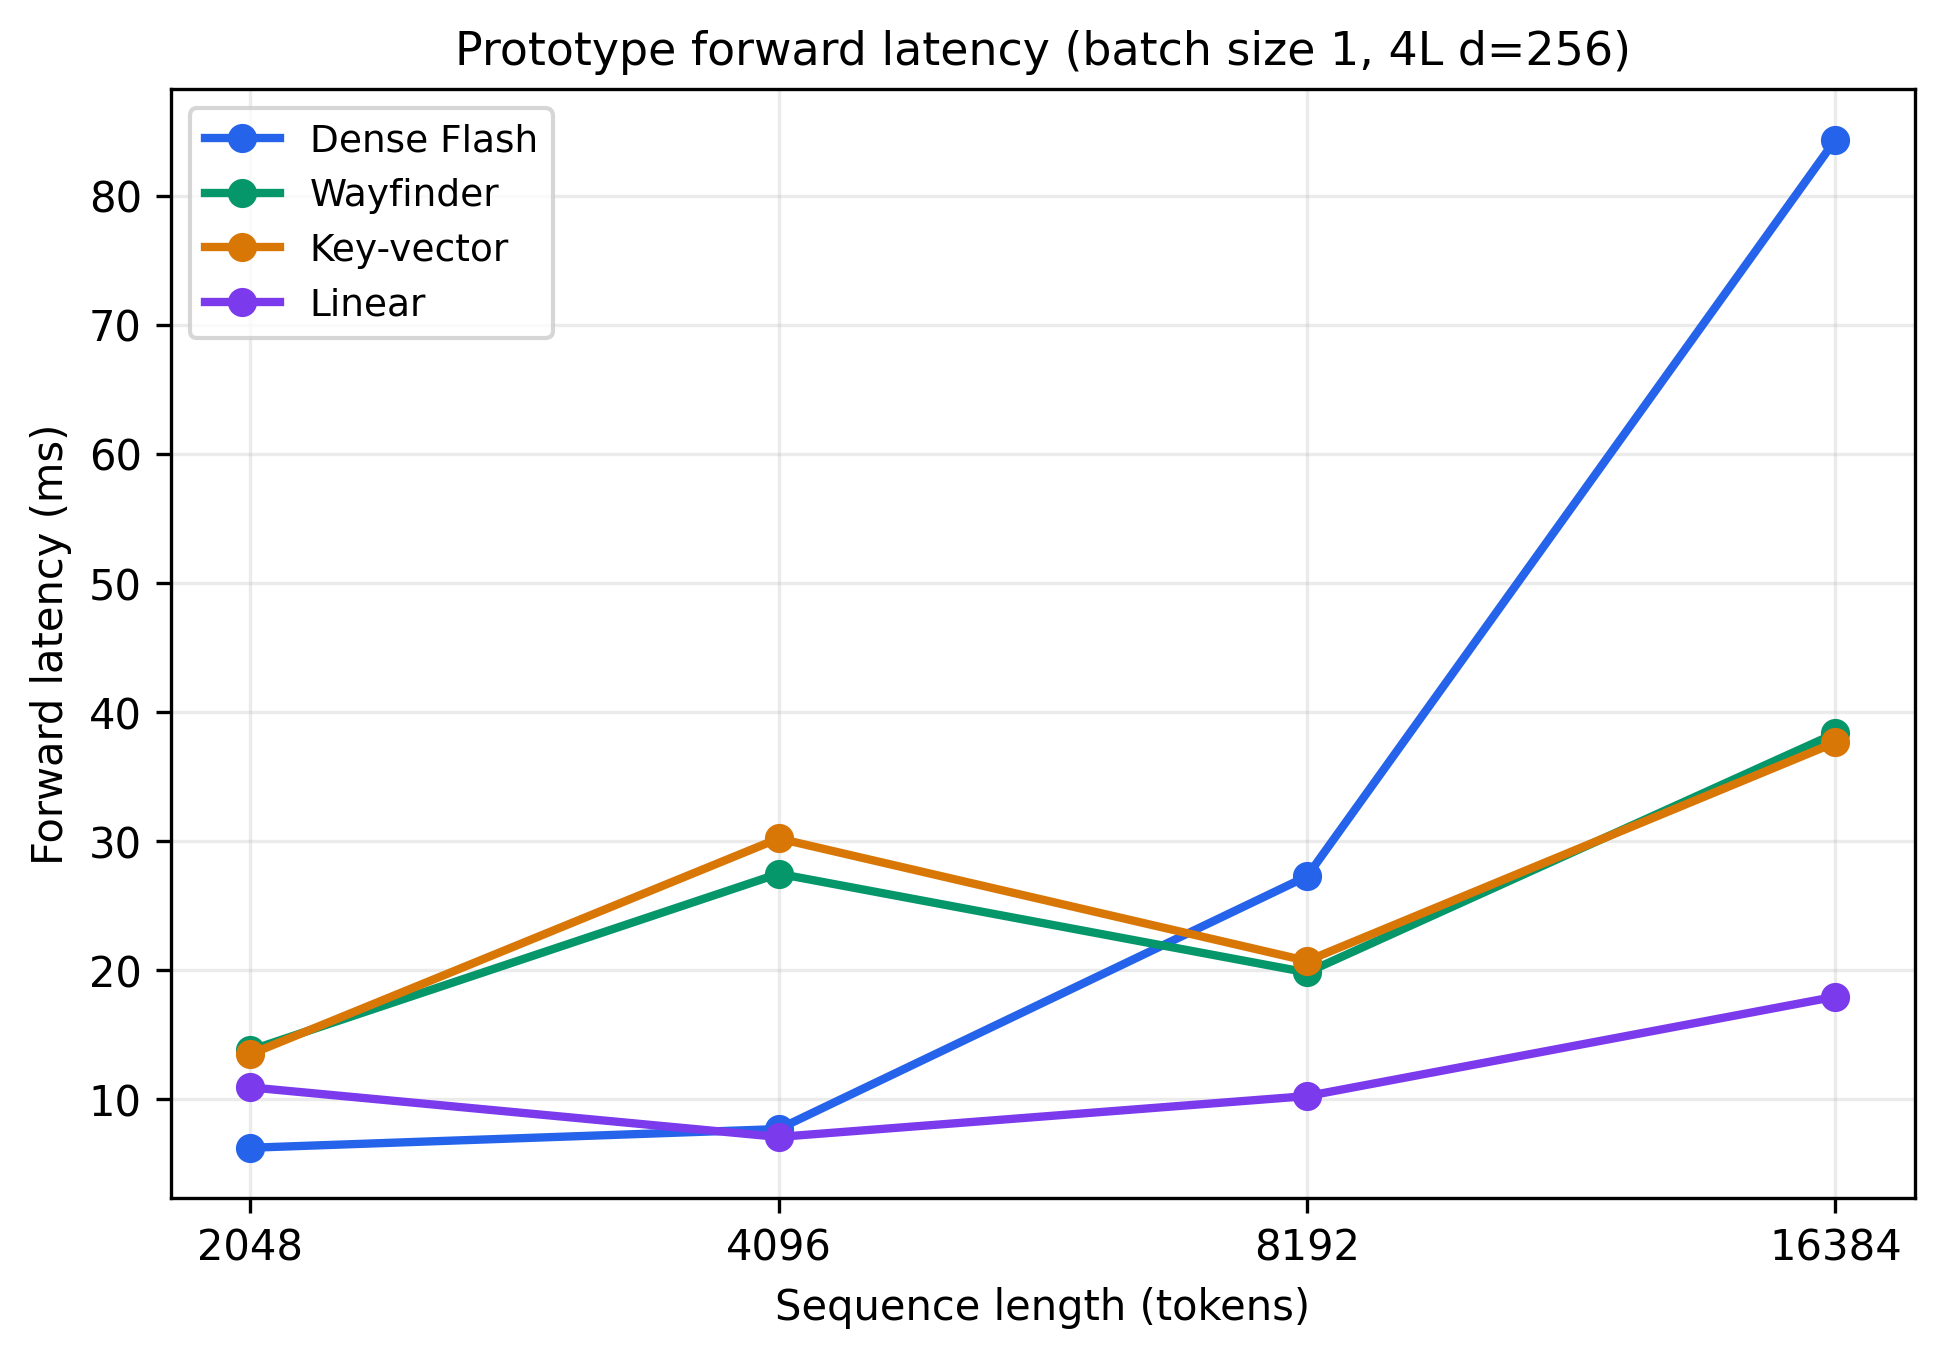
\includegraphics[width=0.86\linewidth]{fig_latency.png}
\caption{Prototype forward latency by sequence length. Dense FlashAttention is faster at short lengths; Wayfinder and key-vector sparse variants cross over at longer lengths; linear attention is fastest in this synthetic benchmark.}
\label{fig:latency}
\end{figure}

At $T{=}16384$, Wayfinder is approximately 2.2$\times$ faster than dense FlashAttention and uses approximately 2.4$\times$ less peak VRAM. Linear attention remains faster and smaller but represents a different tradeoff: global-state compression rather than learned sparse retrieval.

\section{Supporting and Negative Results}

\subsection{Early index-quality experiments}

Before the main NIAH experiments, we evaluated index-learning variants on an MNIST pixel-LM setup. Table~\ref{tab:mnist-index} summarizes Recall@32 results.

\begin{table}[H]
\caption{Early routing and index-quality experiments on MNIST pixel-LM teacher attention. The random Recall@32 baseline is approximately 17\% for this MNIST $T=784$ setup.}
\centering
\small
\begin{tabular}{lc}
\toprule
Variant & Mean Recall@32 \\
\midrule
Asymmetric RouterMLP & 60.6 \\
Learned-address & 57.2 \\
Key-vector baseline & 52.4 \\
Symmetric reference & 45.3 \\
Per-head supervision & 39.3 \\
Joint auxiliary loss & 25.3 \\
MSE attention regression & 15.4 \\
\bottomrule
\end{tabular}
\label{tab:mnist-index}
\end{table}

These experiments motivated two design choices: asymmetric query/key geometry and InfoNCE-style ranking loss. MSE attention regression failed badly, landing below the random Recall@32 baseline for that MNIST cache setting.

\subsection{MNIST task gate}

In the MNIST task-gate experiment, sparse variants were stable with similar task performance; the dense baseline collapsed after extended fine-tuning (26.6\% digit accuracy, LM loss 1.70 vs.\ roughly 94--95\% and loss near 0.87 for sparse variants). Because dense was not a valid quality ceiling, we do not use this as main evidence---only as a diagnostic that Recall@K differences need not translate into task separation.

\subsection{Decoy curriculum}

Table~\ref{tab:decoy} summarizes a harder decoy curriculum using an asymmetric sparse-routing variant from a separate suite---not our canonical Wayfinder training path. It is included as an important limitation.

\begin{table}[H]
\caption{Decoy curriculum at $T{=}2048$. Routing variant from the decoy suite, not the canonical Wayfinder path.}
\centering
\small
\begin{tabular}{lccccc}
\toprule
Decoys & Dense & Linear & Routing variant & Local $W=64$ & Local $W=256$ \\
\midrule
0 & 100.0 & 100.0 & 99.7 & 13.3 & 48.0 \\
1 & 56.7 & 62.3 & 42.0 & 12.3 & 30.7 \\
2 & 41.7 & 53.0 & 25.0 & 12.3 & 26.7 \\
4 & 26.7 & 36.3 & 22.7 & 12.3 & 20.7 \\
\bottomrule
\end{tabular}
\label{tab:decoy}
\end{table}

This is a strong limitation: we do not establish superiority over linear attention. On decoy variants, linear outperformed dense and the routing variant, motivating future work on multi-hop retrieval, language modeling, and harder retrieval settings.

\subsection{Layerwise address diagnostics}

The aggregate index diagnostic in the main results hides depth across transformer layers. Table~\ref{tab:layerwise} reports layerwise Wayfinder Recall@32 after Phase B; the sparse forward pass nevertheless uses $K=128$.

\begin{table}[H]
\caption{Layerwise Wayfinder address Recall@32 in the 2048-token proof-cell diagnostic.}
\centering
\small
\begin{tabular}{lc}
\toprule
Layer & Wayfinder Recall@32 \\
\midrule
0 & 31.1 \\
1 & 57.9 \\
2 & 67.0 \\
3 & 81.5 \\
\bottomrule
\end{tabular}
\label{tab:layerwise}
\end{table}

\subsection{Failed protocols excluded from main claims}

Several runs are excluded from main evidence tables. From-scratch long-context training without our recipe collapsed to near-chance at $T \ge 4096$. A seed-reproduction suite with a broken protocol similarly failed. Dry-run artifacts with tiny budgets are software validation only. These negative results motivated the final recipe but are not evidence for the main quantitative claim.

\section{Discussion}

\subsection{What has been shown?}

The evidence supports:
\begin{itemize}
    \item \textbf{Recipe.} Dense teacher neighborhoods distill into asymmetric token-level addresses via multi-positive InfoNCE on teacher top-32 neighborhoods, followed by sparse fine-tuning; the recipe recovers dense-quality behavior on easy NIAH through $T{=}4096$, training without it collapsed in excluded runs, and Phase B Recall@32 is a weak proxy for final accuracy after Phase C.
    \item \textbf{Mechanism ablation.} At $T{=}2048$ with matched $K{=}128$, dedicated addresses outperform key-vector top-$K$ sparsification (100.0\% vs.\ 81.3\%); fixed local windows fail when the needed token lies outside the window.
    \item \textbf{Distillation objective.} Contrastive ranking over teacher neighborhoods outperforms full attention-matrix MSE for index learning on MNIST caches.
    \item \textbf{Index diagnostic.} Teacher-neighborhood Recall@$K$ can diverge from downstream sparse-attention accuracy when search and aggregation geometries differ.
    \item \textbf{Systems prototype.} Fused exact causal retrieval plus sparse QKV readout crosses over dense FlashAttention at long context in forward-pass benchmarks, enabled by sparse $\mathcal{O}(T K d_h)$ QKV work, exact low-$d_A$ address search with fused tiling, and prototype kernels---not sublinear approximate retrieval.
\end{itemize}
These results complement frontier learned-index systems such as DSA \cite{deepseek2025v32} by isolating a minimal mechanism, controlled ablations, and explicit diagnostics rather than claiming production-scale LM performance.

\subsection{What has not been shown?}

The evidence does not support universal superiority over linear attention. Linear matches dense on easy NIAH and outperforms dense in the decoy curriculum---a strong baseline and often a better speed-quality point on these synthetic tasks.

\paragraph{Where Wayfinder and linear may diverge.}
Linear attention summarizes the prefix into a fixed-size global state---efficient but not selective. Wayfinder targets sparse, query-specific lookup followed by softmax over retrieved tokens. We expect divergence on tasks with many retrievable bindings, multi-hop lookup, or content-addressable recall where a global linear state poorly proxies ``which past tokens matter.'' Our main NIAH setting is intentionally easy (one needle, zero decoys) and does not stress-test that distinction.

We conjecture that where (i) dense beats linear because content-selective long-range lookup matters and (ii) exact dense attention is too costly, Wayfinder may offer sparse retrieval closer to dense behavior at sub-quadratic cost. Testing on TinyStories-scale LMs and multi-binding synthetic tasks is future work.

\subsection{Why the training recipe matters}

Failed runs trained variants from scratch at long context without dense-teacher initialization, address-index pretraining, and sparse fine-tuning collapsed to near-chance at $T \ge 4096$. The recipe is part of the method, not an implementation detail: dense attention discovers a retrieval graph, InfoNCE distills it into an index, and sparse fine-tuning adapts the model to the retrieved neighborhood.

\section{Limitations}

\paragraph{Compute scope.}
All main results used a single RTX 5090 (32GB) under WSL. Trained Wayfinder quality is reported through $T=4096$. Broader evaluations (TinyStories LMs, RULER-style multi-key retrieval, one-decoy cells under our recipe, multi-seed reproduction) were deferred to finish the controlled NIAH study at $T \le 4096$---not for lack of hardware in principle, but because each benchmark repeats the full training pipeline on a single GPU.

Important limitations:
\begin{itemize}
    \item The main benchmark is synthetic pointer retrieval, not real language modeling.
    \item Results are primarily from one canonical seed.
    \item Forward-pass systems benchmarks at 8192 and 16384 use $T \le 4096$ weights with extended position embeddings; they measure latency and memory, not trained retrieval quality at those lengths.
    \item Linear attention is faster and matches or exceeds dense on several synthetic settings.
    \item The decoy curriculum uses a different routing path, not our canonical Wayfinder recipe.
    \item The current systems implementation is a prototype.
    \item Index diagnostics use Recall@32 for Wayfinder and Recall@128 for key-vector on the same holdout cache; a same-$K$ diagnostic sweep was not completed.
    \item Linear systems latency was measured in a separate session from the dense/Wayfinder/key-vector table, although harness and model config match.
    \item Direct experimental comparisons against BigBird, Reformer, Performer, Routing Transformer, BiFormer, Native Sparse Attention, LHA, DSA, HashAttention, SeerAttention, Quest, and Saap have not yet been run in this codebase.
\end{itemize}

\section{Future Work}

\paragraph{End-to-end learned indexing.}
A natural extension is joint address-index training during dense pretraining: start dense, gradually add address InfoNCE, then anneal to top-$K$ sparse attention. Untested so far.

\paragraph{Harder retrieval cells.}
A concrete next step is the one-decoy hard cell under our canonical Wayfinder recipe. The decoy results here used a different routing path and should not be treated as final learned-address performance under distractors.

\paragraph{Broader benchmarks.}
Evaluate Wayfinder against linear attention on language modeling, RULER-style multi-key retrieval, multi-hop synthetic retrieval, and long-context documents, emphasizing settings where selective retrieval---not global compression---is the bottleneck.

\paragraph{Approximate causal retrieval.}
At very large $T$, exact fused causal top-$K$ search may dominate runtime despite low $d_A$. Off-the-shelf ANN libraries such as FAISS are a poor fit for the canonical in-layer problem as implemented today: token addresses change every forward, causality requires per-query filtering, and our experimental FAISS path paid GPU--CPU transfer, per-forward index rebuild, and Python post-filtering costs that exceeded fused GPU causal top-$K$. A more promising systems direction is therefore \emph{GPU-native} approximate causal retrieval---persistent or incrementally updated indexes, HNSW/IVF or learned LSH over token addresses with fused causal filtering---trading sublinear query cost against recall and downstream task accuracy rather than assuming ANN recall matches dense teacher neighborhoods.

\paragraph{Learned indices beyond attention.}
Our study isolates in-layer token-address retrieval; the same search-then-read decomposition may apply to mixture-of-experts routing, external memory, KV-cache pruning, and agent memory.

\paragraph{Learned graph search (speculative).}
Dense causal attention can be viewed as one-step message passing over a complete directed token graph. Wayfinder makes the search step explicit but still performs one-hop top-$K$ retrieval over the causal prefix. A more ambitious long-term direction is \emph{learned graph-search attention}: tokens would induce a sparse dynamic graph (learned edges plus optional structural biases), queries would enter through address similarity and expand through a small number of hops, and standard softmax QKV readout would run only over the reached frontier. Such a model might better match compositional multi-hop lookup than one-hop search, and could in principle reduce search cost below exact prefix MIPS, but it introduces hard training and systems problems---discrete traversal, per-layer graph dynamics, and the risk of collapsing back to ordinary top-$K$ sparsification on simple retrieval tasks. We treat this as speculation beyond the scope of this study.

\section{Conclusion}

We studied how to distill dense causal attention into learned-address sparse attention. A dense teacher discovers useful neighborhoods; contrastive training of asymmetric addresses learns to retrieve them; sparse fine-tuning jointly adapts the index and standard attention pathway for softmax over the retrieved set. The design follows learned decoupled sparse indexing \cite{sun2022lha,deepseek2025v32,desai2025hashattention,mazare2025saap}, including frontier systems such as DSA, but our evidence is narrow: a reproducible recipe; a matched-budget ablation where dedicated addresses match dense while key-vector top-$K$ fails at $T{=}2048$; MNIST evidence favoring InfoNCE over full-matrix MSE; a diagnostic where Recall@$K$ misleads; and prototype long-context crossover over dense FlashAttention. Results do not show universal dominance over linear attention; they support the thesis that this distillation recipe and decoupled addresses recover dense behavior where key-vector top-$K$ routing cannot, in a reproducible small-scale setting.

\section*{Acknowledgments}

Experiments were run on a single NVIDIA RTX 5090 (32GB) under WSL. Figures in \texttt{paper\_figures/} were generated by \texttt{scripts/generate\_wayfinder\_paper\_figures.py} from canonical result artifacts. Primary proof-cell outputs: \texttt{experiments/Experiment\_7/learned\_address\_proof\_cell/proof\_cell\_full/}.

\begin{thebibliography}{99}

\bibitem{vaswani2017attention}
Ashish Vaswani, Noam Shazeer, Niki Parmar, Jakob Uszkoreit, Llion Jones, Aidan N. Gomez, Lukasz Kaiser, and Illia Polosukhin.
Attention Is All You Need.
In Advances in Neural Information Processing Systems, 2017.

\bibitem{dao2022flashattention}
Tri Dao, Daniel Y. Fu, Stefano Ermon, Atri Rudra, and Christopher Re.
FlashAttention: Fast and Memory-Efficient Exact Attention with IO-Awareness.
In Advances in Neural Information Processing Systems, 2022.

\bibitem{dao2024flashattention2}
Tri Dao.
FlashAttention-2: Faster Attention with Better Parallelism and Work Partitioning.
In International Conference on Learning Representations, 2024.

\bibitem{beltagy2020longformer}
Iz Beltagy, Matthew E. Peters, and Arman Cohan.
Longformer: The Long-Document Transformer.
arXiv:2004.05150, 2020.

\bibitem{zaheer2020bigbird}
Manzil Zaheer, Guru Guruganesh, Avinava Dubey, Joshua Ainslie, Chris Alberti, Santiago Ontanon, Philip Pham, Anirudh Ravula, Qifan Wang, Li Yang, and Amr Ahmed.
Big Bird: Transformers for Longer Sequences.
In Advances in Neural Information Processing Systems, 2020.

\bibitem{kitaev2020reformer}
Nikita Kitaev, Lukasz Kaiser, and Anselm Levskaya.
Reformer: The Efficient Transformer.
International Conference on Learning Representations, 2020.

\bibitem{roy2021routing}
Aurko Roy, Mohammad Saffar, Ashish Vaswani, and David Grangier.
Efficient Content-Based Sparse Attention with Routing Transformers.
Transactions of the Association for Computational Linguistics, 2021.

\bibitem{zhu2023biformer}
Lei Zhu, Xinjiang Wang, Zhanghan Ke, Wayne Zhang, and Rynson W. H. Lau.
BiFormer: Vision Transformer with Bi-Level Routing Attention.
In IEEE/CVF Conference on Computer Vision and Pattern Recognition, 2023.

\bibitem{yuan2025nsa}
Jingyang Yuan, Huazuo Gao, Damai Dai, Junyu Luo, Liang Zhao, Zhengyan Zhang, Zhenda Xie, Yuxing Wei, Lean Wang, Zhiping Xiao, Yuqing Wang, Chong Ruan, Ming Zhang, Wenfeng Liang, and Wangding Zeng.
Native Sparse Attention: Hardware-Aligned and Natively Trainable Sparse Attention.
In Proceedings of the 63rd Annual Meeting of the Association for Computational Linguistics (Volume 1: Long Papers), pages 23078--23097, Vienna, Austria. Association for Computational Linguistics, 2025. doi:10.18653/v1/2025.acl-long.1126.

\bibitem{wang2020linformer}
Sinong Wang, Belinda Z. Li, Madian Khabsa, Han Fang, and Hao Ma.
Linformer: Self-Attention with Linear Complexity.
arXiv:2006.04768, 2020.

\bibitem{choromanski2021performer}
Krzysztof Choromanski, Valerii Likhosherstov, David Dohan, Xingyou Song, Andreea Gane, Tamas Sarlos, Peter Hawkins, Jared Davis, Afroz Mohiuddin, Lukasz Kaiser, David Belanger, Lucy Colwell, and Adrian Weller.
Rethinking Attention with Performers.
International Conference on Learning Representations, 2021.

\bibitem{lewis2020rag}
Patrick Lewis, Ethan Perez, Aleksandra Piktus, Fabio Petroni, Vladimir Karpukhin, Naman Goyal, Heinrich K\"uttler, Mike Lewis, Wen-tau Yih, Tim Rockt\"aschel, Sebastian Riedel, and Douwe Kiela.
Retrieval-Augmented Generation for Knowledge-Intensive NLP Tasks.
In Advances in Neural Information Processing Systems, 2020.

\bibitem{johnson2019faiss}
Jeff Johnson, Matthijs Douze, and Herv\'e J\'egou.
Billion-scale Similarity Search with GPUs.
IEEE Transactions on Big Data, 7(3):535--547, 2021.

\bibitem{malkov2018hnsw}
Yu. A. Malkov and D. A. Yashunin.
Efficient and Robust Approximate Nearest Neighbor Search Using Hierarchical Navigable Small World Graphs.
IEEE Transactions on Pattern Analysis and Machine Intelligence, 42(4):824--836, 2020.

\bibitem{oord2018cpc}
Aaron van den Oord, Yazhe Li, and Oriol Vinyals.
Representation Learning with Contrastive Predictive Coding.
arXiv:1807.03748, 2018.

\bibitem{chen2020simclr}
Ting Chen, Simon Kornblith, Mohammad Norouzi, and Geoffrey Hinton.
A Simple Framework for Contrastive Learning of Visual Representations.
In Proceedings of the 37th International Conference on Machine Learning, pages 1597--1607, 2020.

\bibitem{radford2021clip}
Alec Radford, Jong Wook Kim, Chris Hallacy, Aditya Ramesh, Gabriel Goh, Sandhini Agarwal, Girish Sastry, Amanda Askell, Pamela Mishkin, Jack Clark, Gretchen Krueger, and Ilya Sutskever.
Learning Transferable Visual Models From Natural Language Supervision.
In Proceedings of the 38th International Conference on Machine Learning, 2021.

\bibitem{sun2022lha}
Zhiqing Sun, Yiming Yang, and Shinjae Yoo.
Sparse Attention with Learning to Hash.
In International Conference on Learning Representations, 2022.

\bibitem{deepseek2025v32}
DeepSeek-AI.
DeepSeek-V3.2: Pushing the Frontier of Open Large Language Models.
arXiv:2512.02556, 2025.

\bibitem{desai2025hashattention}
Aditya Desai, Shuo Yang, Alejandro Cuadron, Matei Zaharia, Joseph E. Gonzalez, and Ion Stoica.
HashAttention: Semantic Sparsity for Faster Inference.
In Proceedings of the 42nd International Conference on Machine Learning, pages 13402--13418, 2025.

\bibitem{mazare2025saap}
Pierre-Emmanuel Mazar\'e, Gergely Szilvasy, Mar\'ia Lomel\'i, Francisco Massa, Naila Murray, Herv\'e J\'egou, and Matthijs Douze.
Inference-Time Sparse Attention with Asymmetric Indexing.
arXiv:2502.08246, 2025.

\bibitem{gao2024seerattention}
Yizhao Gao, Zhichen Zeng, Dayou Du, Shijie Cao, Peiyuan Zhou, Jiaxing Qi, Junjie Lai, Hayden Kwok-Hay So, Ting Cao, Fan Yang, and Mao Yang.
SeerAttention: Learning Intrinsic Sparse Attention in Your LLMs.
arXiv:2410.13276, 2024.

\bibitem{tang2024quest}
Jiaming Tang, Yilong Zhao, Kan Zhu, Guangxuan Xiao, Baris Kasikci, and Song Han.
Quest: Query-Aware Sparsity for Efficient Long-Context LLM Inference.
In Proceedings of the 41st International Conference on Machine Learning, 2024.

\bibitem{lou2024sparsek}
Chao Lou, Zixia Jia, Zilong Zheng, and Kewei Tu.
Sparser is Faster and Less is More: Efficient Sparse Attention for Long-Range Transformers.
arXiv:2406.16747, 2024.

\bibitem{liu2024retrievalattention}
Di Liu, Meng Chen, Baotong Lu, Huiqiang Jiang, Zhenhua Han, Qianxi Zhang, Qi Chen, Chengruidong Zhang, Bailu Ding, Kai Zhang, Chen Chen, Fan Yang, Yuqing Yang, and Lili Qiu.
RetrievalAttention: Accelerating Long-Context LLM Inference via Vector Retrieval.
arXiv:2409.10516, 2024.

\bibitem{mohtashami2023landmark}
Amirkeivan Mohtashami and Martin Jaggi.
Landmark Attention: Random-Access Infinite Context Length for Transformers.
In Advances in Neural Information Processing Systems, 2023.

\bibitem{piekos2025mosa}
Piotr Pi\k{e}kos, R\'obert Csord\'as, and J\"urgen Schmidhuber.
Mixture of Sparse Attention: Content-Based Learnable Sparse Attention via Expert-Choice Routing.
arXiv:2505.00315, 2025.

\bibitem{sundarapandiyan2025fsa}
Vijaykaarti Sundarapandiyan, Tom Goldstein, and Ashwinee Panda.
Foreign Sparse Attention: Effective Distillation into Sparse Attention.
In ICML Workshop on Efficient Systems for Foundation Models (ES-FoMo III), 2025.

\bibitem{fu2026sparda}
Yaosheng Fu, Guangxuan Xiao, Xin Dong, Song Han, and Oreste Villa.
SparDA: Sparse Decoupled Attention for Efficient Long-Context LLM Inference.
arXiv:2606.04511, 2026.

\end{thebibliography}

\end{document}
